 % arara: clean: { files: [thesis.aux, thesis.bbl, thesis.blg, thesis.dvi, thesis.fdb_latexmk, thesis.fls, thesis.idx, thesis.ilg, thesis.ind, thesis.lof, thesis.log, thesis.lot, thesis.nlo, thesis.nls, thesis.out, thesis.pdf, thesis.ps, thesis.toc]}
% arara: latex:  { shell: yes }
% arara: bibtex
% arara: nomencl
% arara: latex
% arara: makeindex
% arara: latex:  { shell: yes }
% arara: dvips
% arara: ps2pdf

% ******************************* PhD Thesis Template **************************
% Please have a look at the README.md file for info on how to use the template

\documentclass[a4paper,12pt,times,numbered,print,index]{Classes/PhDThesisPSnPDF}

% ******************************************************************************
% ******************************* Class Options ********************************
% *********************** See README for more details **************************
% ******************************************************************************

% `a4paper'(The University of Cambridge PhD thesis guidelines recommends a page
% size a4 - default option) or `a5paper': A5 Paper size is also allowed as per
% the Cambridge University Engineering Deparment guidelines for PhD thesis
%
% `11pt' or `12pt'(default): Font Size 10pt is NOT recommended by the University
% guidelines
%
% `oneside' or `twoside'(default): Printing double side (twoside) or single
% side.
%
% `print': Use `print' for print version with appropriate margins and page
% layout. Leaving the options field blank will activate Online version.
%
% `index': For index at the end of the thesis
%
% `draft': For draft mode without loading any images (same as draft in book)
%
% `draftmode': Special draft mode with line numbers, images, and water mark with
% timestamp and custom text. Position of the text can also be modified.
%
% `abstract': To generate only the title page and abstract page with
% dissertation title and name, to submit to the Student Registry
%
% `chapter`: This option enables only the specified chapter and it's references
%  Useful for review and corrections.
%
% ************************* Custom Page Margins ********************************
%
% `custommargin`: Use `custommargin' in options to activate custom page margins,
% which can be defined in the preamble.tex. Custom margin will override
% print/online margin setup.
%
% *********************** Choosing the Fonts in Class Options ******************
%
% `times' : Times font with math support. (The Cambridge University guidelines
% recommend using times)
%
% `fourier': Utopia Font with Fourier Math font (Font has to be installed)
%            It's a free font.
%
% `customfont': Use `customfont' option in the document class and load the
% package in the preamble.tex
%
% default or leave empty: `Latin Modern' font will be loaded.
%
% ********************** Choosing the Bibliography style ***********************
%
% `authoryear': For author-year citation eg., Krishna (2013)
%
% `numbered': (Default Option) For numbered and sorted citation e.g., [1,5,2]
%
% `custombib': Define your own bibliography style in the `preamble.tex' file.
%              `\RequirePackage[square, sort, numbers, authoryear]{natbib}'.
%              This can be also used to load biblatex instead of natbib
%              (See Preamble)
%
% **************************** Choosing the Page Style *************************
%
% `default (leave empty)': For Page Numbers in Header (Left Even, Right Odd) and
% Chapter Name in Header (Right Even) and Section Name (Left Odd). Blank Footer.
%
% `PageStyleI': Chapter Name next & Page Number on Even Side (Left Even).
% Section Name & Page Number in Header on Odd Side (Right Odd). Footer is empty.
%
% `PageStyleII': Chapter Name on Even Side (Left Even) in Header. Section Number
% and Section Name in Header on Odd Side (Right Odd). Page numbering in footer


% ********************************** Preamble **********************************
% Preamble: Contains packages and user-defined commands and settings
% ******************************************************************************
% ****************************** Custom Margin *********************************

% Add `custommargin' in the document class options to use this section
% Set {innerside margin / outerside margin / topmargin / bottom margin}  and
% other page dimensions
\ifsetCustomMargin
  \RequirePackage[left=37mm,right=30mm,top=35mm,bottom=30mm]{geometry}
  \setFancyHdr % To apply fancy header after geometry package is loaded
\fi

% *****************************************************************************
% ******************* Fonts (like different typewriter fonts etc.)*************

% Add `customfont' in the document class option to use this section

\ifsetCustomFont
  % Set your custom font here and use `customfont' in options. Leave empty to
  % load computer modern font (default LaTeX font).
  \RequirePackage{libertine}
\fi

% *****************************************************************************
% **************************** Custom Packages ********************************



% ************************* Algorithms and Pseudocode **************************

%\usepackage{algpseudocode}


% ********************Captions and Hyperreferencing / URL **********************

% Captions: This makes captions of figures use a boldfaced small font.
%\RequirePackage[small,bf]{caption}

\RequirePackage[labelsep=space,tableposition=top]{caption}
\renewcommand{\figurename}{Fig.} %to support older versions of captions.sty


% *************************** Graphics and figures *****************************

%\usepackage{rotating}
%\usepackage{wrapfig}

% Uncomment the following two lines to force Latex to place the figure.
% Use [H] when including graphics. Note 'H' instead of 'h'
%\usepackage{float}
%\restylefloat{figure}

% Subcaption package is also available in the sty folder you can use that by
% uncommenting the following line
% This is for people stuck with older versions of texlive
%\usepackage{sty/caption/subcaption}
\usepackage{subcaption}

% ********************************** Tables ************************************
\usepackage{booktabs} % For professional looking tables
\usepackage{multirow}

%\usepackage{multicol}
%\usepackage{longtable}
%\usepackage{tabularx}


% ***************************** Math and SI Units ******************************

\usepackage{amsfonts}
\usepackage{amsmath}
\usepackage{amssymb}
\usepackage{enumitem}
\usepackage{siunitx} % use this package module for SI units


% ******************************* Line Spacing *********************************

% Choose linespacing as appropriate. Default is one-half line spacing as per the
% University guidelines

% \doublespacing
% \onehalfspacing
% \singlespacing


% ************************ Formatting / Footnote *******************************

%\usepackage[perpage]{footmisc} %Range of footnote options


% *****************************************************************************
% *************************** Bibliography  and References ********************

%\usepackage{cleveref} %Referencing without need to explicitly state fig /table

% Add `custombib' in the document class option to use this section
\ifuseCustomBib
   \RequirePackage[square, sort, numbers, authoryear]{natbib} % CustomBib

% If you would like to use biblatex for your reference management, as opposed to the default `natbibpackage` pass the option `custombib` in the document class. Comment out the previous line to make sure you don't load the natbib package. Uncomment the following lines and specify the location of references.bib file

% \RequirePackage[backend=biber, style=numeric-comp, citestyle=numeric, sorting=nty, natbib=true]{biblatex}
% \bibliography{References/references} %Location of references.bib only for biblatex

\fi


% changes the default name `Bibliography` -> `References'
\renewcommand{\bibname}{References}


% *****************************************************************************
% *************** Changing the Visual Style of Chapter Headings ***************
% This section on visual style is from https://github.com/cambridge/thesis

% Uncomment the section below. Requires titlesec package.

%\RequirePackage{titlesec}
%\newcommand{\PreContentTitleFormat}{\titleformat{\chapter}[display]{\scshape\Large}
%{\Large\filleft{\chaptertitlename} \Huge\thechapter}
%{1ex}{}
%[\vspace{1ex}\titlerule]}
%\newcommand{\ContentTitleFormat}{\titleformat{\chapter}[display]{\scshape\huge}
%{\Large\filleft{\chaptertitlename} \Huge\thechapter}{1ex}
%{\titlerule\vspace{1ex}\filright}
%[\vspace{1ex}\titlerule]}
%\newcommand{\PostContentTitleFormat}{\PreContentTitleFormat}
%\PreContentTitleFormat


% ******************************************************************************
% ************************* User Defined Commands ******************************
% ******************************************************************************

% *********** To change the name of Table of Contents / LOF and LOT ************

%\renewcommand{\contentsname}{My Table of Contents}
%\renewcommand{\listfigurename}{My List of Figures}
%\renewcommand{\listtablename}{My List of Tables}


% ********************** TOC depth and numbering depth *************************

\setcounter{secnumdepth}{2}
\setcounter{tocdepth}{2}


% ******************************* Nomenclature *********************************

% To change the name of the Nomenclature section, uncomment the following line

%\renewcommand{\nomname}{Symbols}


% ********************************* Appendix ***********************************

% The default value of both \appendixtocname and \appendixpagename is `Appendices'. These names can all be changed via:

%\renewcommand{\appendixtocname}{List of appendices}
%\renewcommand{\appendixname}{Appndx}

% ******************************** Draft Mode **********************************

% Uncomment to disable figures in `draftmode'
%\setkeys{Gin}{draft=true}  % set draft to false to enable figures in `draft'

% These options are active only during the draft mode
% Default text is "Draft"
%\SetDraftText{DRAFT}

% Default Watermark location is top. Location (top/bottom)
%\SetDraftWMPosition{bottom}

% Draft Version - default is v1.0
%\SetDraftVersion{v1.1}

% Draft Text grayscale value (should be between 0-black and 1-white)
% Default value is 0.75
%\SetDraftGrayScale{0.8}


% ************************ Thesis Information & Meta-data **********************
% Thesis title and author information, refernce file for biblatex
% ************************ Thesis Information & Meta-data **********************
%% The title of the thesis
\title{An executable stochastic model for Fatty Acid metabolism}
%\texorpdfstring is used for PDF metadata. Usage:
%\texorpdfstring{LaTeX_Version}{PDF Version (non-latex)} eg.,
%\texorpdfstring{$sigma$}{sigma}

%% Subtitle (Optional)

%% The full name of the author
\author{Argyris Zardilis}

%% Department (eg. Department of Engineering, Maths, Physics)
\dept{Department of Applied Mathematics and Theoretical Physics}

%% University and Crest
\university{University of Cambridge}
\crest{
\includegraphics[width=0.25\textwidth]{University_Crest}}

%% You can redefine the submission text:
% Default as per the University guidelines: This dissertation is submitted for
% the degree of Doctor of Philosophy
%\renewcommand{\submissiontext}{change the default text here if needed}

%% Full title of the Degree
\degree{Master of Philosophy}

%% College affiliation (optional)
\college{St Catharine's College}

%% Submission date
% Default is set as {\monthname[\the\month]\space\the\year}
%\degreedate{2014} 

%% Meta information
\subject{LaTeX} \keywords{{LaTeX} {PhD Thesis} {Engineering} {University of
Cambridge}}


% ***************************** Abstract Separate ******************************
% To printout only the titlepage and the abstract with the PhD title and the
% author name for submission to the Student Registry, use the `abstract' option in
% the document class.

\ifdefineAbstract
 \pagestyle{empty}
 \includeonly{Declaration/declaration, Abstract/abstract}
\fi

% ***************************** Chapter Mode ***********************************
% The chapter mode allows user to only print particular chapters with references
% Title, Contents, Frontmatter are disabled by default
% Useful option to review a particular chapter or to send it to supervisior.
% To use choose `chapter' option in the document class

\ifdefineChapter
 \includeonly{Chapter3/chapter3}
\fi

% ******************************** Front Matter ********************************
\begin{document}

\frontmatter

\begin{titlepage}

\maketitle

\end{titlepage}

% ******************************* Thesis Dedidcation ********************************



% ******************************* Thesis Declaration ********************************

\begin{declaration}

I hereby declare that except where specific reference is made to the
work of others, the contents of this dissertation are original and
have not been submitted in whole or in part for consideration for any
other degree or qualification in this, or any other university. This
dissertation is the result of my own work and includes nothing which
is the outcome of work done in collaboration, except where
specifically indicated in the text. This dissertation contains fewer
than 18,000 words including captions, footnotes and headers.

% Author and date will be inserted automatically from thesis.tex \author \degreedate

\end{declaration}


% ************************** Thesis Acknowledgements *****************************

\begin{acknowledgements}      


And I would like to acknowledge ...


\end{acknowledgements}

% ************************** Thesis Abstract *****************************
% Use `abstract' as an option in the document class to print only the titlepage and the abstract.
\begin{abstract}
Metabolites and reactions taking part in Lipid metabolism processes
are often poorly annotated. This makes it difficult to analyse with
current traditional techniques used for metabolic processes like Flux
Balance Analysis (FBA). Moreover because of the low number of carbons flowing
towards Lipid metabolism pathways the effect of the inherent
probabilistic nature of chemical events is amplified. This behaviour
is then not very well described by the average deterministic view
offered by FBA. Here we propose an alternative stochastic
reaction-centric view of Lipid metabolism to
better capture some of its defining characteristics on a more local
scale: iterative conversion processes, probabilistic decisions, and
crucial regulatory mechanisms. Regulatory mechanisms are thought to be
tightly regulated and their disruption leads to loss of metabolic
balance that seems to be consistent with disorders. 
We also assess the formal graphical
language of Petri Nets to capture this stochastic reaction-centric
view and contrast it with the pi-calculus process algebra that is
another popular approach for executable models in Biology.  Here we
particularly focus on Fatty Acid (FA) synthesis that is a core part of
lipid metabolism. A basic high-level Petri Net and stochastic
pi-calculus model for the FA
synthesis/elongation presented along with techniques for tuning it with
experimental datasets. The Petri Net model is then further extended to include
an important  regulatory mechanism of FA synthesis activity through
the action of AMPK protein kinase.
\end{abstract}


% *********************** Adding TOC and List of Figures ***********************

\tableofcontents

\listoffigures

\listoftables

% \printnomenclature[space] space can be set as 2.5cm between symbol and
% description

% ******************************** Main Matter *********************************
\mainmatter


%*****************************************************************************************
%*********************************** First Chapter ***************************************
%*****************************************************************************************

\chapter{Introduction}  %Title of the First Chapter

\ifpdf
    \graphicspath{{Chapter1/Figs/Raster/}{Chapter1/Figs/PDF/}{Chapter1/Figs/}}
\else
    \graphicspath{{Chapter1/Figs/Vector/}{Chapter1/Figs/}}
\fi

Recent technological advances which led to an accumulation
of a wealth of data that have made Biology as a
discipline shift some of its efforts from understanding individual
components to understanding systems of interacting components. A
systems level understanding is really important
as it is the distributed information processing that gives rise to phenotype and the macroscopic
behaviour of cells to sustain life. Biology as a discipline has not traditionally used
any formal methods but as the systems under investigation grow in size,
more formal approaches are needed. System Biology is a relatively
new field that tries to fill the gap by bringing practises from
traditionally more formal disciplines like Mathematics, Physics, and
Computer Science \cite [] {ideker2001new}.

In the area of metabolism, we have gone from a study of the properties
of single enzymes and metabolites to the study of the behaviour of
entire metabolic pathways and even entire genome-wide metabolisms
of mammalian and model organisms. This accumulated knowledge about the
interconnections in and between metabolic pathways is deposited in
large online databases that integrate the information from various
sources. While these diagrams are a rich source of information
since metabolism is a highly dynamic process sometimes a more dynamic
picture is needed. Mathematical techniques like Flux Balance analysis
originating from Dynamical Systems Theory are particularly popular in
the analysis of the flows in and out of metabolic pathways.

Recently the biochemical reasons behind
different diseases were pinpointed  in the loss of balance between anabolic and catabolic
activities in cells. Most of these activities are known to be tightly
regulated to avoid excess production and accumulation of metabolites
which can be the reasons behind observed disorders. The products and
intermediaries of lipid metabolism are central in many metabolic
disorders and diseases. While Flux Balance
Analysis is of great importance in the study of large metabolic
networks it is not so suited in studying more local probabilistic metabolic
processes and their crucial regulatory mechanisms.

Here we propose an alternative reaction-centric and stochastic view of metabolic
systems and lipid metabolism in particular which we think will be an important tool in the mechanistic
characterisation of crucial local metabolic processes and their
regulatory mechanisms. We also propose the formal language of Petri
Nets, which has been successfully used before in biochemical networks,
as a potential tool to capture this alternative reaction-centric view
of lipid metabolism. The goals and the work done towards this project were therefore two-fold:
Firstly create a reaction-centric model of the Fatty Acid(FA)
synthesis/elongation process which is an important part of lipid
metabolism and secondly assess the formal modelling language of Petri
Nets as a potential tool to capture this view. Since part of the work
done was about modelling methodology and since we noticed a more
general trend towards executable formal models in biology \cite [] {fisher2007executable} we also
present here an alternative version of the model in the process
algebra of  pi-calculus in an attempt to contrast the two formal
modeling approaches: net models and process algebra models.

In this introduction I start by introducing the currently most popular
methodology for the description of metabolic pathways(FBA),
outline the biological importance of lipid metabolism and the
motivation for a reaction-centric view, and finally I try to place
Petri Nets and pi-calculus(the two methodologies used) in the spectrum
of formal
distributed computing modelling language world.

\section{Dynamical systems theory and Flux Balance Analysis}
Systems Biology attempts to master the complexity and understand metabolic
pathways and any biological system by usually contructing
models. There are two types of models based on their construction
method. Bottom-up models are constructed by extracting biological
knowledge from experimental datasets. This category includes for
example the diagrammatic means of capturing the interconnected
structure of metabolic pathwayw. Top-down models on the other hand
start from a detailed knowledge of the system to get a mechanistic
model of the system \cite [] {schneider2013understanding}.

Early attemps to capture the interactions and dependencies between
components were made with bottom-up models which resulted in large diagrams that
capture the conversion processes happending inside metabolic pathways. While these
diagrams are important and are a useful represntation of our knowledge
about metabolism they lack the dynamic nature which is crucial in a
systems level understanding of a system which should not only include
the connections between the components but also how these components
interact over time, how their behaviour is
controlled, and how they respond to external stimuli \cite [] {kitano2002systems}.

\begin{figure}[htbp!]
\centering
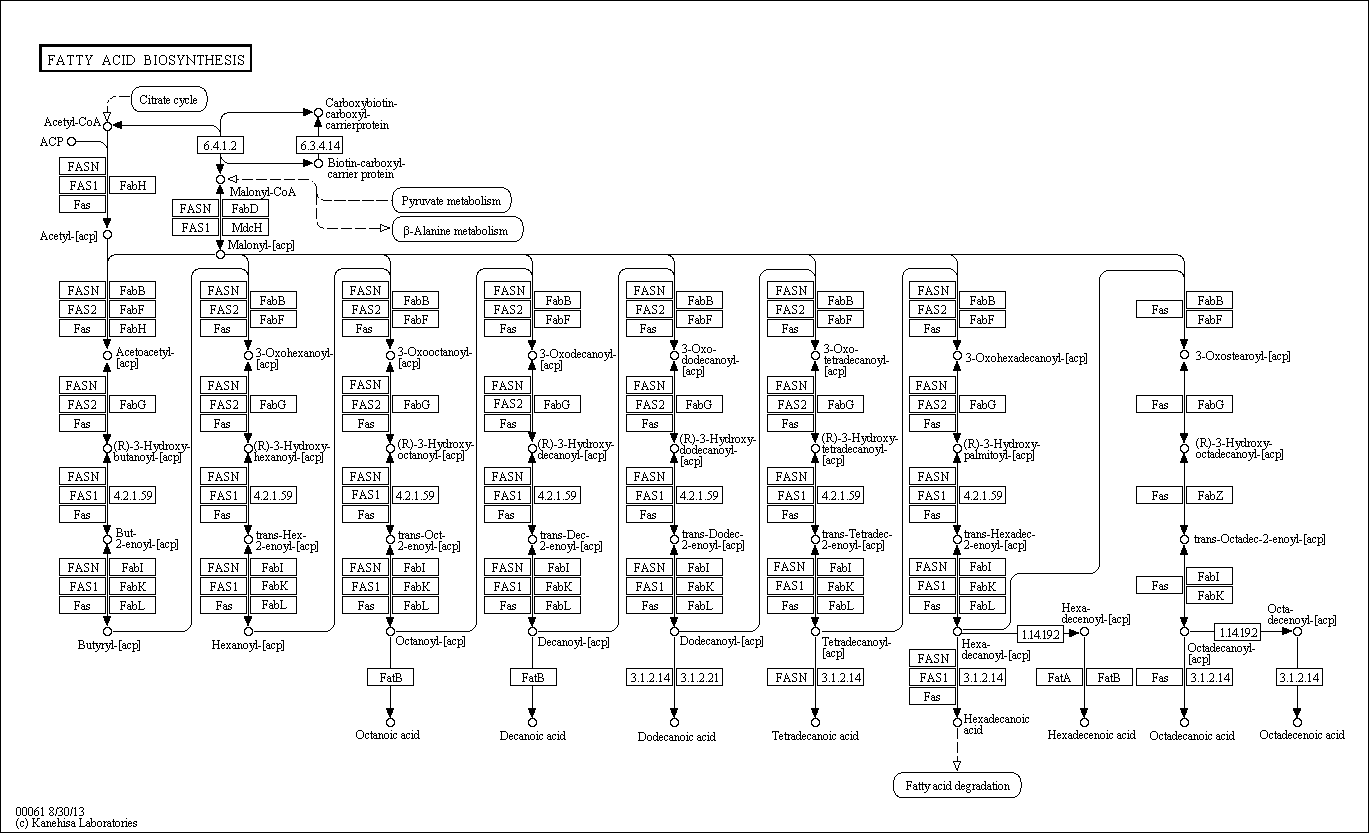
\includegraphics[width=1.0\textwidth]{fa_synthesis_pathway}
\caption[Fatty Acid synthesis pathway]{Fatty acid synthesis pathway
  captured by the standard diagrammatic language used to capture
  interactions between components in a biological system. This was
  taken from KEGG a database which contains current knowledge about
  the working of these systems(from experiments for example)
  integrated with data from multiple sources.}
\label{fig:fa_synthesis_pathway}
\end{figure}

This need to look into dynamic behaviour led to Dynamical System
theory which based on its success in Physics has found its way in many
other fields. Dynamical system theory captures the relationship
between continuous quantities in difference-differential equations
which describe the evolution of state variables in terms of changes
in other state variables and even themselves thus capturing the
interaction element. Since the time of Newton and classical mechanics
,where these ideas originated, the toolbox of dynamical systems theory
has grown to include techniques for qualitative understanding of
system without the need to solve them either numerically or
analytically.

In biochemistry each species in the system is represented by its
concentration leading to a differential equation for each species. The
rate of change of the concentration of a species is described in terms
of in flows- increasing the rate of change(production)- and out flows
- decreasing the rate of change(degradation). These flows can be
dependent on the concentrations of other variables(species) which
participate in the same biochemical reactions. Consider for example a
system with $n$ components which we can group into the global state of
the system $\mathbf{x} = (x_1, x_2, \dots x_n)$. All the reactions
that take place in the system change, in discrete levels, the numbers
of molecules of the species:

\begin{align*}
\mathbf{x} &\overset{r_1(\mathbf{x})}{\longrightarrow} \mathbf{x} +
\mathbf{\delta_1}\\
\mathbf{x} &\overset{r_2(\mathbf{x})}{\longrightarrow} \mathbf{x} +
\mathbf{\delta_2}\\
\vdots \\
\mathbf{x} &\overset{r_m(\mathbf{x})}{\longrightarrow} \mathbf{x} +
\mathbf{\delta_m}
\end{align*}
So for every reaction we have one such rule and $\delta_k$ are the
discrete levels by which the species change for every reaction. Each
reaction has an associated and possible state dependent rate $r_k(x)$
which is the expected number of times it takes place in a time
unit. The in-flows are the positive deltas and out-flows the negative
ones. The differential equation describing the evolution of the average numbers
of  species $i$ is then the sum of the in
and out flows over all reactions in the system:

\begin{equation*}
\frac{dx_i}{dt} = \sum_{m} r_m(\mathbf{x})\delta_{mi}
\end{equation*}

Usually this formulation of the problem leads to integration with a
numerical ODE solver of the above system to get the dynamic behaviour
of the system. The usual problem mathematical biologists face is that
the reaction rate function(the $r_k(\mathbf{x})$s) contain parameter
constants that are not usually known.

In the contex of metabolic systems however there is a mathematical technique however, called Flux Balance
Analysis, that is used to compute these flows without explicit
knowledge of these parameters by making some assumptions about the
system to simplify the problem \cite [] {orth2010flux}. If we assume that that metabolites
cannot accumulate within the cell and their levels are more or less
balanced then the system is at steady-state. The steady-state assumption means that the average positive flux-defined as the sum of
all the in-flows- and the average negative flux-defined as the sum of
all the out-flows- are equal which in turn means that the rate of
change for every species , defined as the sum of all flows(negative and
positive), is equal to 0. Solving for the fluxes leads to a linear equation for each
species. For a more concise notation all the $\delta_{nm}$ are
packaged into a matrix $\mathbf{S}$, traditionally called the Stoichiometric
matrix, and the fluxes in a vector $\mathbf{r}$. Then the problem
becomes solving the system $\mathbf{Sr} = \mathbf{0}$ to calculate the
fluxes $\mathbf{r}$ through our system of interest. The only problem
with this formulation of the problem is that the system is
underdetermined since usually the number of reactions is higher than
the number of species. To solve this the solution space is constrained
with the use of an objective function which leads to a linear
programming problem formulation which is easily solvable. An small
contrived example to illustrate the above process is given in
Figure~\ref{fig:fba}.

\begin{figure}[htbp!]
\centering
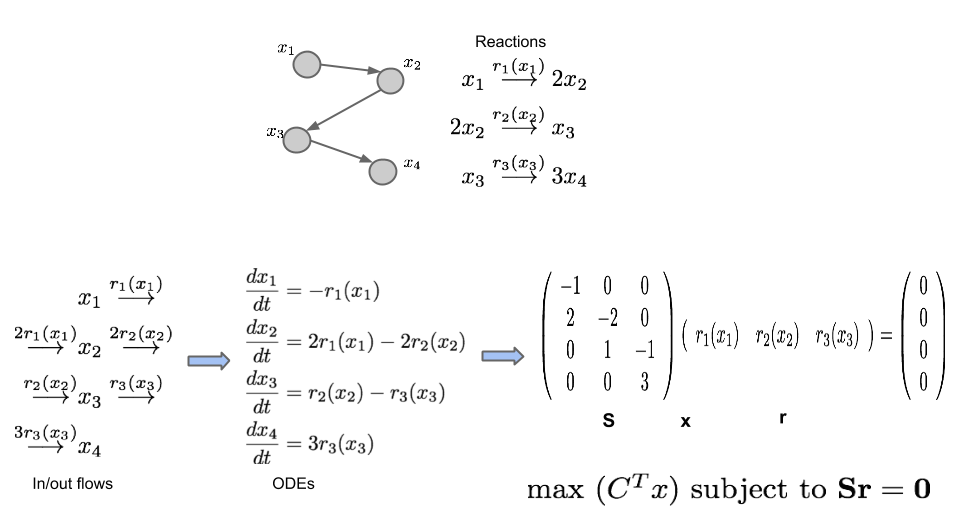
\includegraphics[width=1.0\textwidth]{fba}
\caption[Flux Balance analysis]{A small example how starting from a
  bottom-up model like a pathway from KEGG we can go on to apply FBA
  and calculate the fluxes through our pathway}
\label{fig:fba}
\end{figure}

Flux balance analysis is a very powerful technique since it allows us
to overcome the problem of the rate function parameters and calculate the
fluxes through the system in a computationally efficient way. It is
not without its limitations though. For large networks of components
finding a suitable objective function to used to transform to solve
the underdetermined problem can be difficult. More importantly and
since it relies on the average behaviour as described by the
differential equations it is not able to capture stochastic,
non-deterministic behaviour.

\section{Challenge of lipid metabolism}
Lipid metabolism is the set of all the anabolic and catabolic
processes that involve lipid products which serve mainly as energy
stores or in the form of lipid bilayers as membranes. The starting
point of lipid metabolism are the Fatty Acids which act as building
blocks for more complex lipids like triacylglycerols. Lipids are
produced by the organism to serve as energy stores in the well-fed state when there is an excess
of carbohydrates and no immediate energy requirements. Any excess
glucose molecules are converted to lipids as follows: When the
glucogen stores are full, glucose molecules will find the way through
the glycolysis pathway blocked at the level of phosphofructokinase so
they take a diversion through the Pentose Phosphate pathway and then
join the glycolytic processes at a later stage bypassing the
block. Then they continue down the normal route to Acetyl-CoA and the
Krebs cycle in the mitochondria. Here since the immediate energy requirements
are low Acetyl-CoA only makes it to the first stage of the Krebs cycle
producing Citrate instead of continuing through the cycle and then to
the Respiratory chain to produce energy. Since Citrate cannot proceed any further in the
cycle its levels accumulate and at some point it diffuses from
the mitochondrion into the cytosol where it is converted to Acetyl-CoA
again to serve as a precursor to Fatty Acid Synthesis which required
the NADPH produced by the Pentose Phosphate pathway. Once Fatty Acid
are synthesised they can go on to form more complex lipid products like
TAGs or get further modified by the Fatty Acid elongation pathway or
by adding bonds to their CH tails. The beta-oxidation pathway in
mitochondria breaks down Fatty Acids into Acetyl-CoA which is then fed
into the Krebs cycle \cite [] {salway2013metabolism}.

\begin{figure}[htbp!]
\centering
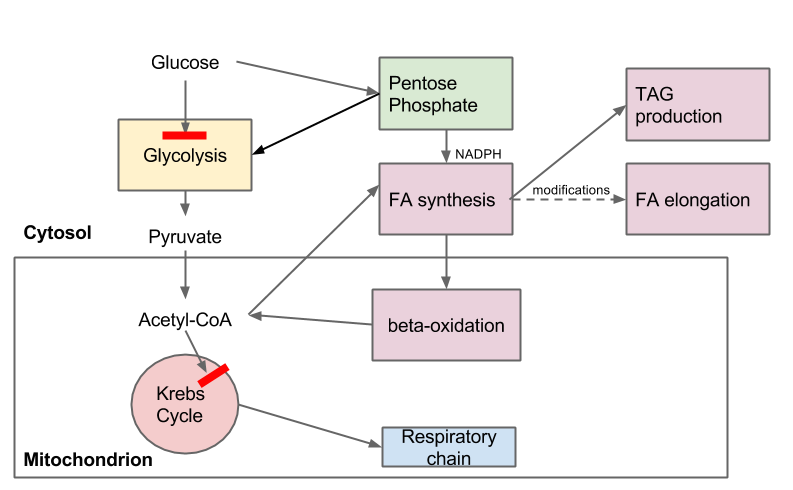
\includegraphics[width=1.0\textwidth]{metabolism}
\caption[Lipid metabolism and interacting pathways]{A diagram
  outlining the main pathways involved in lipid metabolism.}
\label{fig:lipid_metabolism}
\end{figure}

All the above production processes have their equivalent catabolic
processes and a balance between the two is essential for metabolic
homeostasis in organisms. This balance is regulated by within and
between pathway control signals which also integrate signals from the
environment. In diseases like type I Diabetes this balance is
disrupted because of insulin deficiency which breaks the regulatory
signals. Fatty Acids and lipid metabolism pathways play a key role
in this chain of disruptions. Also, free Fatty acids are
associated with obesity and type II diabetes \cite [] {boden2002free}.

We notice from the above brief overview and the pictorial description
of the interconnected pathways(Figure~\ref{fig:lipid_metabolism}) that
in metabolism and lipid metabolism products flow through the
network with an iterative chain-like conversion process and that at
several points there are probabilistic decisions to be made for the next step in the
chain. These decisions are tightly regulated by signals from other
pathways and the environment and disruption of these signals is
observed in diseases like Diabetes. It is important therefore to have
a mechanistic explanation of the 'trip' through the metabolic chain
and the non-deterministic 'decision-making' that happens and its regulation. We believe
that in order to get this mechanistic characterisation we would
benefit from a stochastic reaction-centric view of lipid metabolism to
give a more local perspective into the iterative conversion processes
and their stochastic nature which stems from the probabilistic
decision-making process. In this study we
focus on the Fatty Acid Biosynthesis pathway which is an important
part of lipid metabolism and it exhibits the characeteristics that are
suited to a reaction-centric analysis: iterative behaviour with
non-deterministic decisions and regulation mechanisms that relate it
to other pathways.

A biochemical system, like the one given in the previous section,
consisting of a number of reactions that alter the integer numbers of
molecules of the species describes a stochastic process and a Continuous
Time Markov Chain in particular. The differential equations we used as
a basis for FBA are a just
deterministic view of the average behaviour. The dynamics of the
system can be set in motion inside a computer using the Gillespie
exact simulation algorithm which creates sample
time-series \cite [] {gillespie1977exact}. Statistical information like the strenth of the
fluctuations (normalised variance) can be computed by collecting a lot
of these traces.

In this study we propose Petri Nets as an alternative language to capture this
reaction-centric view which we think is more expressive than the
standard Markov processes formulation. While Petri Nets and their
evolution through their formal operational semantics also describe a
CTMC and are thus equivalent in power with the standard Markov jump
processes we believe that they posses some characteristics(see next
section and Methods) that makes them useful in the analysis of the
reaction-centric view of lipid metabolism. Language is important not
only because a syntax is needed to define our models in but also because
the notation we use is our tool of thought and the use of the correct
language for thinking about a problem can enhance our understadnding
and ultimately help us solving it \cite [] {iverson2007notation}. That is why we have more
than one high-level programming language despite the fact that all of
them are Turing complete and therefore have the ability to express all
computations.

In the next section we try to place Petri Nets, the main modelling
language used, and pi-calculus, the alternative used as a way to
contrast net and process algebras models, in the spectra of formal
modelling methodologies for distributed computation.

\section{Computational models in Biology}
Computer Science, although a fundamentally different discipline than
Biology, has undergone a similar transformation in its focus from
single information processing entities to systems of interacting
entities(see the Internet, clusters). The term computation at the
distributed level is now broader; it not only describes mere
calculation but it also includes the interaction between
components. This change in the term computation can be seen through
the models we use to capture the notion of computation. At the early
days of computing(even before actual electronic computers) the models
of computation included lambda-calculus and Turing Machines. These
early formalisms capture computation differently, Turing Machine as
global state transitions in an Abstract Machine and lambda-calculus
as reduction rules in a calculus, but they are effectively equivalent
in expressive power(see Church-Turing thesis). As computer systems
grew there was an interest for similar
minimalistic languages to express distributed computation. Some
formalisms that were invented during that period were
\citet{milner1980calculus} Calculus of Communicating Systems,
\citet{lafont1989interaction} Interaction nets,
\citet{milner1992calculus} pi-calculus, and Petri
Nets \cite [] {murata1989petri}.

The analogy between distributed computer systems and biochemical
systems was made explicit by \citet{berry1989chemical} and the
Chemical Abstract Machine. The modelling langugages used for
distributed computation are applicalbe in biological systems since
they both include a high number of concurrent components with dependencies
introducing non-deterministic behaviour. \citet{fontana1996barrier} went as far as
to propose pi-calculus as an alternative to dynamical systems
theory since he considered a calculus of objects that can change and their
interactions more appropriate for describing biochemical systems than a calculus of continuous
interacting quantities. \citet{priami2001application} went on to use a
stochastic version of pi-calculus to describe a biochemical systems
and from then on other Computer Science inspired formalisms came up like
\citet{cardelli2005brane} with Brane-calculi, \citet{danos2004formal}
with kappa, and
\citet{ciocchetta2009bio} with Bio-PEPA.

Petri Nets lean towards the automata and Turing Machines style of
computation because their operational semantics are in terms of state
transitions from a distributed global state. They have a very intuitive
graphical notation and concurrency,
non-determinism, and the causal independencies between events is
inherent in their structure. They
also have a very natural correspondence to biochemical reactions and
in their basic form have been used mainly to capture qualitative properties
of biochemical systems \cite [] {baldan2010petri}. In this study we use the stochastic version of
Petri Nets which explicitly models time to describe and quantitatively
analyse the
reaction-centric view of the FA elongation and synthesis
process.

Process algebras, which pi-calculus is an example of, on the other
hand define syntax to specify the behaviour and state transitions of the individual
components of the system independently therefore reactions and
compositionality are not explicitly captured. In this study I
particularly use Stochastic Pi Machine (SPiM) which is a programming
language derived from stochastic pi-calculus but extended to include
operational semantics for execution on an Abstract Machine and also a
formal graphical notation \cite [] {export:65224, export:65223}. The
fact that this variant shares
characteristics from both net models and process algebras approached
makes it an interesting case-study.

\section{Outline of work}
To summarise the main aim of this study was to assess the
applicability of the Petri net formal language to capture a
reaction-centttric view of lipid metabolism by producing a model of the
Fatty Acid biosyntesis/elongation process. For completeness we also
created a stochastic pi-calculus version of the model to contrast the
two methodologies as part of the more general turn towards executable
formal models in Biology. An extended version of the basic process is
also given including part of its regulatory mechanisms.

In chapter~\ref{chap:methods} an overview of the methods used in
modelling the process is given, namely Petri Nets and stochastic
pi-calculus. In section~\ref{chap:work} the basic and extended model
are presented along with their tuning with available metabolomics
data. Finally in section~\ref{chap:discussion}


%*****************************************************************************************
%*********************************** Second Chapter **************************************
%*****************************************************************************************

\chapter{Methods}
\label{chap:methods}
\ifpdf
    \graphicspath{{Chapter2/Figs/Raster/}{Chapter2/Figs/PDF/}{Chapter2/Figs/}}
\else
    \graphicspath{{Chapter2/Figs/Vector/}{Chapter2/Figs/}}
\fi

\section{Data sources}

\section{Petri Nets}
\subsection{Syntax and Semantics of Basic nets}
A Petri Net is a 4-tuple $(P, T, pre, post)$ defined as:
\begin{itemize}
\item[-] a set of \textit{places} (or conditions) $P$
\item[-] a set of \textit{transitions} (or events) $T$
\item[-] a \textit{preconditions map pre} : $T \rightarrow \mathbf{m}P$ which assigns a multiset of places $pre(t)$ to each transition $t \in T$
\item[-] a \textit{postconditions map post} : $T \rightarrow \mathbf{m}P$ which assigns a multiset of places $post(t)$ to each transition $t \in T$
\end{itemize}
where $\mathbf{m}P$ is the space of multisets over $P$ with a multiset over P defined as function $f: P \rightarrow \mathbb{N}$. The state of the system, called a marking, is again a multiset $\mathcal{M}$ over $P$. We can think of the marking as the distributed global state of the system. It is also common when defining a Petri Net to give the initial marking of the system usually written as $\mathcal{M}_0$.

The operational semantics of Petri Nets is defined in terms of changes in the global state through the action of 
the transitions $T$ of the PN:
\begin{equation*}
\mathcal{M}\overset{t}{\longrightarrow}\mathcal{M^\prime}
\end{equation*}
Here when a transition(event) $t$ occurs it changes the state of the system from marking $\mathcal{M}$ to marking $\mathcal{M^\prime}$. Unlike automata and Turing Machines however a transition does not occur from a single global state but instead it only affects part of the state:
\begin{equation*}
\mathcal{M}\overset{t}{\longrightarrow}\mathcal{M^\prime} \mbox{ iff } pre(t) \leq \mathcal{M} \mbox{ and } \mathcal{M^\prime} = \mathcal{M} - pre(t) + post(t)
\end{equation*}
For 2 multisets $f$ and $g$ over set $X$, $f \leq g$ is defined as $f \leq g \iff \forall x \in X f_x \leq g_x$. So a transition $t$ is said to be 'enabled' if its preconditions are sufficiently marked($pre(t) \leq \mathcal{M}$) and when it 'fires' it changes the marking in the places in its vicinity, namely the set of places $\{p \mbox{ }|\mbox{ } pre(t)_p \neq 0 \mbox{ or } post(t)_p \neq 0\}$($\mathcal{M^\prime} = \mathcal{M} - pre(t) + post(t)$). 
The \textit{post} and \textit{pre} condition maps define the causal independence between transitions and add the ability of Petri Nets to model concurrency and non-determinism. Two (or more) transitions are concurrent if they do not share any preconditions. Non-determinism is added through dependencies of transitions which share preconditions. In that case a race condition is created because the dependent transitions compete at their shared preconditions with only one of them being able to fire at each step. 

This formal definition of transitions leads to an algorithm for the executions of a PN as follows:
\begin{enumerate}[noitemsep]
\item Initialise the net  with $(P, T, pre, post)$ and set state $\mathcal{M} = \mathcal{M}_0$
\item Find enabled transitions, $enabled \subseteq T, \forall t \in T \mbox{ if } pre(t) \leq M$
\item Choose transition $t$ from set of enabled at random
\item Update state according to $\mathcal{M} = \mathcal{M} -pre(t) + post(t)$
\item Repeat steps 2-4 until there are no more enabled transitions or an external stop condition is met(e.g. max number of steps)
\end{enumerate}

The main strength of Petri Nets though lies on their very intuitive and widely used graphical representation. Petri Nets are represented as bipartite graphs with two sets of nodes, the places $P$ and transitions $T$ which are denoted by circles and rectangles respectively. A weighted directed edge with weight $n>0$ is added between place $p$ and transition $t$ in the direction $p\rightarrow t$ if $pre(t)_p=n$. A weighted directed edge with weight $n>0$ is added between transition $t$ and place $p$ in the direction $t\rightarrow p$ if $post(t)_p=n$. The markings are denoted as dots (tokens) in the circles depicting the places. So for example consider the net with $P=\{p1, p2, p3\}$, $T=\{t1\}$, $pre=\{(t1, \{(p1, 2), (p2, 1), (p3, 0)\})\}$, $post=\{(t1, \{(p1, 0), (p2, 0), (p3, 2)\})\}$, and marking $\{(p1, 3), (p2, 1), (p3, 1)\}$. The graphical depiction of this net would be the one shown in Figure \ref{fig:pn_example}. We could then also define the pre-places of a transition $t$ as all the places $p$ such that $pre(t)_p >0 $ and the post-places as all the places $p$ such that $post(t)_p >0 $.

\begin{figure}
\centering

\includegraphics[scale=1.0]{pn_example}
\caption{Small basic Petri Net example}
\label{fig:pn_example}
\end{figure}

The operational semantics of Petri Nets can also be defined very naturally in this graphical notation. When a transition $t$ fires $pre(t)_p$ tokens are consumed from all the pre-places $p$ and $post(t)_p$ tokens are added to all the post-places $p$. For the net given above(Figure \ref{fig:pn_example}) when transition $t1$ fires the 2 tokens are removed from $p1$ and 1 from $p2$ and 2 are added to $p3$(see Figure \ref{fig:pn_operation}).The execution of the net can be seen as the flow of tokens through the net as transitions fire at each step according to the execution algorithm given above. This graphical view of the execution is called the 'token game' and it is very useful for gaining an insight into the dynamic behaviour of the system being modelled.
\begin{figure}
\centering
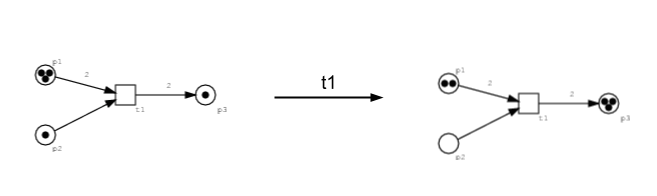
\includegraphics[scale=0.7]{pn_operation}
\caption{The token game for basic Petri Nets.}
\label{fig:pn_operation}
\end{figure}

\subsection{Stochastic Petri Net extension}
Stochastic Petri Nets are an extension to the original Petri Net formalism to explicitly model time. Notice that
even though the there is an ordering of transitions implied by their execution according to the algorithm given 
in the previous section the concept of time is not modelled explicitly in the basic Petri Net formalism. In order
to model time explicitly Stochastic Petri Nets (SPNs) introduce a waiting time associated with each transition $t$, defined as random variable $X_t$ distributed exponentially with potentially marking-dependent rate $\lambda_t(pre\_places(t))$ where $pre\_places$ is defined as before. Formally a SPN is a 5-tuple $(P, T, pre, post, \nu)$ with everything defined as before with the addition of the map $\nu : T \rightarrow H$ where $H$ is the set of all hazard functions $H = \{h_t\mbox{ }|\mbox{ } h_t: \mathbb{N}^{|pre(t)|} \rightarrow \mathbb{R}\}$.
Hazard function is the typical name used in stochastic processes for the function giving the rate of the exponential time variable. In this case the hazard function $h_t$ gives $\lambda_t$ and the domain of $h_t$ we will restrict to only the marking of the pre-places of $t$. This wait time associated with each transition changes the execution algorithm for Petri Nets; now when more than one transition is enabled a wait time is sampled from all of them and the one with the least waiting time gets to fire:
\begin{enumerate}[noitemsep]
\item Initialise the net  with $(P, T, pre, post, \nu)$, set state $\mathcal{M} = \mathcal{M}_0$, and $time=0$
\item Find enabled transitions, $enabled \subseteq T, \forall t \in T \mbox{ if } pre(t) \leq M$
\item For each enabled transition $t$ sample a wait time from an exponential distribution with rate $\lambda_t(pre\_places(t))$. Pick the transition $t_i$ with least wait time to fire.
\item Proceed time $time = time + \tau_i$
\item Update state according to $\mathcal{M} = \mathcal{M} -pre(t_i) + post(t_i)$
\item Repeat steps 2-4 until there are no more enabled transitions or an external stop condition is met(e.g. max number of steps)
\end{enumerate}
With this new variant of Petri Nets we maintain the non-determinism through the competition of enabled transitions with shared preconditions but by changing their rates we can favour some transitions over others. This Stochastic Petri Net formulation gives rise to Continuous Time Markov Chain and the execution algorithm defined above is more or less the Gillespie algorithm which is an exact algorithm for simulation of Markov jump processes. It is this Petri Net variant that we will use to model our system of interest, the Fatty Acid synthesis/elongation pathway. In the next section we describe the correspondence between a biochemical network and especially a metabolic pathway to a Stochastic Petri Net and some examples of previous uses of SPNs in biology/biochemistry.
\subsection{Application to Biochemistry}
The correspondence between a biochemical system and a Stochastic Petri Net is as follows: the chemical species of the system become places, reactions become transitions and their rates the rates of the transitions, and the stoichiometry of the reactions is represented in the \textit{pre} and \textit{post} maps. This is a very natural correspondence between chemical reactions and Petri Nets. In fact the standard notation for chemical notation is itself a process algebra albeit not a very formal one. So for example consider a made-up reaction that takes 2 molecules of A and 3 molecules of B and produces 5 molecules of C:
\begin{equation*}
A + B \overset{r_1}{\longrightarrow} 2C
\end{equation*}

This is an event, a reaction with rate $k$, which tells us how the state of the system changes but although implicitly we know the conditions for it to take place they are not formally captured by the informal process algebra of chemical reactions as defined by the standard arrow notation. A Petri Net representation of this reaction however captures the reaction more formally:


\section{Stochastic Pi-calculus}
This is going to contain a vey brief introduction to stochasic pi-calculus.


\chapter{Work}
\label{chap:work}
% **************************** Define Graphics Path **************************
\ifpdf
    \graphicspath{{Chapter3/Figs/Raster/}{Chapter3/Figs/PDF/}{Chapter3/Figs/}}
\else
    \graphicspath{{Chapter3/Figs/Vector/}{Chapter3/Figs/}}
\fi

The aim of this study was to capture the iterative elongation process
of even-chain saturated Fatty Acids. Fatty Acids are
carboxylic acids with long hydrocarbon side groups
(Figure~\ref{fig:fas}) and they are usually characterised by the
number of carbons in these side-groups, for example a FA with a chain
of 6 carbons is usually denoted as $C_6$. The side-chains of FAs grow
by successive $C_2$ concatenations. This concatenation process takes places at
the FA biosynthesis pathway in the cytosol for chain lengths up to
$C_{18}$. Further elongation takes places at the FA elongation
pathway in the Endoplasmatic Reticulum(ER).

\begin{figure}[htbp!]
\centering
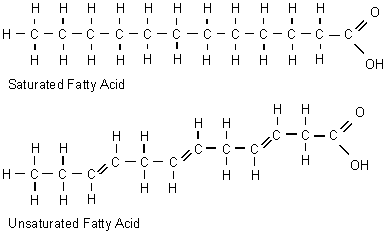
\includegraphics[width=0.6\textwidth]{fas}
\caption[Fatty Acid structure]{The structure of Fatty Acids(FA) which
  consists of a long hydrocarbon side-group. The length of this
  side-group charactersises the FA.}
\label{fig:fas}
\end{figure}

In this study we are interested in the elongation process in its
entirety so our models capture the combined effect of the two pathways
responsible for it, FA biosynthesis \textit{and} FA elongation. In
this section I first introduce the basic model and the assumptions
made to simplify it, the tuning of that basic model based on FA
measurements, a version of the model in stochastic pi-calculus and
finally the extension of the model with the introduction of some
control mechanisms.

\section{Basic model}
\subsection{Petri Net implementation}
FA biosynthesis starts with Acetyl-CoA which is being converted to
Malonyl-CoA. A reaction between Malonyl-CoA and Acetyl-CoA starts off
the first $C_4$ FA product. After that there are successive $C_2$
concatenations to elongate the FA product with each elongation step
, that requires 4 reactions, requiring another Malonyl-CoA(Figure~\ref{fig:fa_synthesis}). The
full pathway from KEGG can be seen in
Figure~\ref{fig:kegg_synthesis}. The elongation pathway located in ER
is similar in nature but the intermediaries are CoAs instead of
ACPs(Figure \ref{fig:kegg_elongation}).

\begin{figure}[htbp!]
\centering
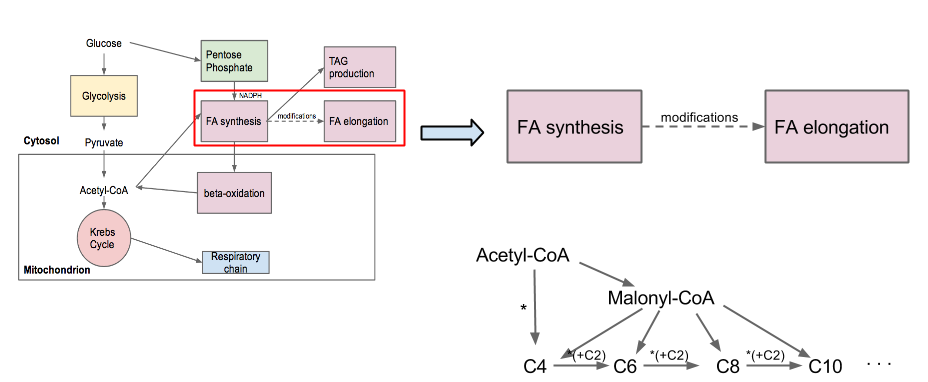
\includegraphics[width=1.0\textwidth]{fa_metabolism}
\caption[FA metabolism]{FA metabolism in relation to other pathways.}
\label{fig:fa_synthesis}
\end{figure}

\begin{figure}[htbp!]
\centering
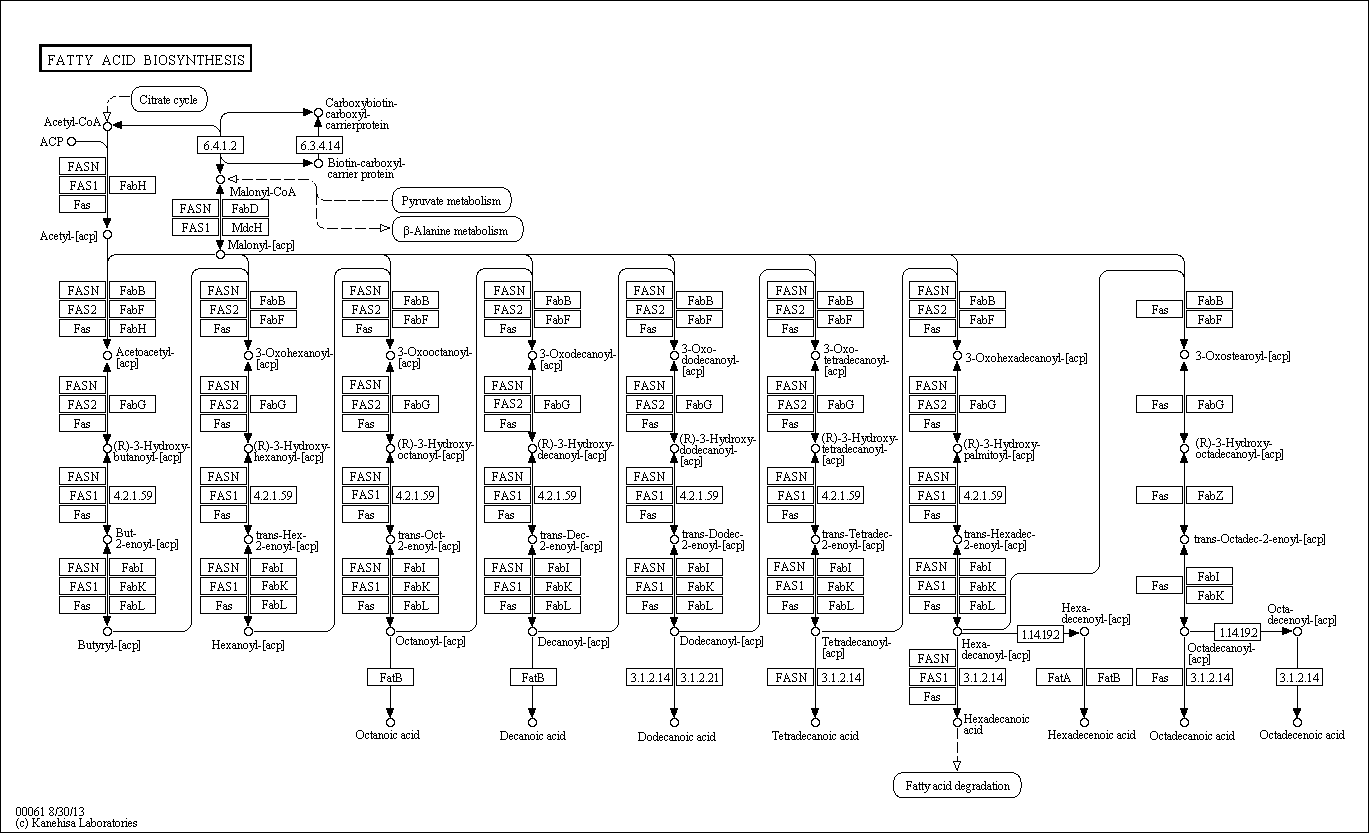
\includegraphics[width=1.0\textwidth]{kegg_synthesis}
\caption[Fatty Acid biosynthsis in cytosol]{FA biosynthesis in the
  cytosol. Notice the successive concatenations. Each concatenation
  takes 4 reactions.}
\label{fig:kegg_synthesis}
\end{figure}

\begin{figure}[htbp!]
\centering
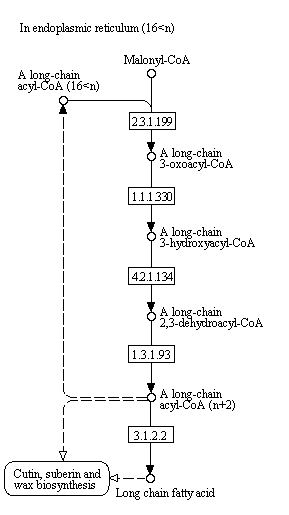
\includegraphics[width=0.3\textwidth]{kegg_elongation}
\caption[Fatty Acid elongation in ER]{General form of FA elongation in
ER. Notice that the intermediate products are CoAs instead of ACPs as
in biosynthesis.}
\label{fig:kegg_elongation}
\end{figure}

Because of the natural correspondence between biochemical reactions as
they are found in the KEGG static model to Petri Net model constructs
a straight translation between the two is straightforward. All the
pathway reactions become transitions with pre-places the reactants and
post-places the products. Here we made our first assumptions by
omitting the enzymes from the reactions. Information about the enzymes
is not so important for our purposes since we are interested in the
numbers of molecules of the metabolites in the system. Information
about the enzymes can be incorporated in the transition rates.
The net can be animated using its formal
operational semantics and as transitions/reactions occur
tokens/metabolites move through the net. The FA products are
represented as sinks, places that are not pre-places to any
transitions, so once a token reaches one of these sinks it is
trapped. That way the probabilistic iterative nature of the process is
capture completely, an intermediate of the process can either remain
at that length or go on to form longer FAs. The sinks are therefore
the outputs of the stochastic process with the inputs being the places
that do not act as post-places for any transitions. Starting with some
finite number of molecules at the inputs, these will be consumed
throughout the process until we reach a dead-state where no further
transitions are enabled. The translation from the KEGG pathway model
to the Petri Net model was done manually with the SNOOPY \cite []
{heiner2012snoopy}tool which
allows you to draw a net and play the token game for basic nets to
observe its behaviour.

\begin{figure}[htbp!]
\centering
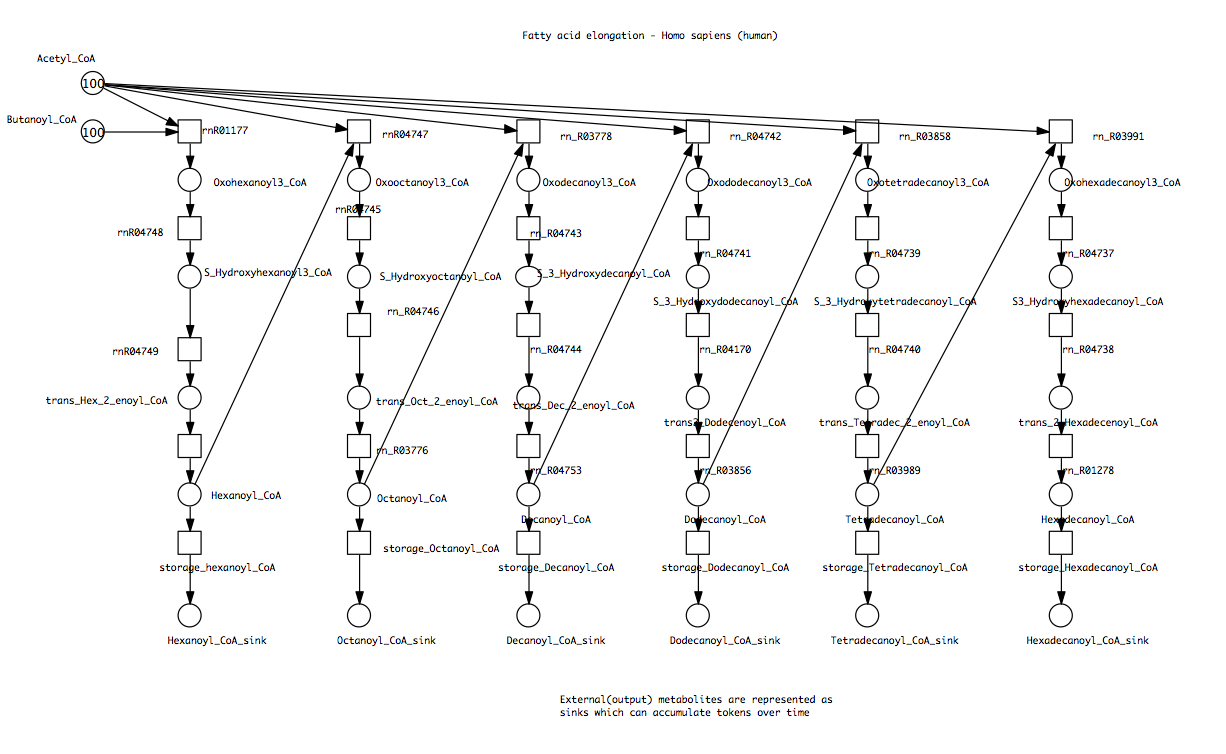
\includegraphics[width=1.0\textwidth]{pn_fa_elongation}
\caption[FA elongation Petri Net model]{}
\label{fig:pn_fa_elongation}
\end{figure}

A direct translation from KEGG is certainly useful for capturing a
low-level biochemical view of the system. The model can offer an even
more fine-control view of the system than the model presented in
Figure~\ref{fig:pn_fa_elongation} by including the enzymes in the
reactions and information about their affinity to the reaction
substrates. However including too many details in the model can
sometimes hide the true aspect of the system the modeller is trying to
understand and analyse. Here we are interested in the probabilistic,
non-deterministic nature of the iterative FA elongation process which
happens as this series of $C_2$ concatenation steps in FA elongation
and biosynthesis pathways in ER and cytosol respectively. The outputs
we are particularly interested to see are the numbers and proportions of FAs at
different lengths. In Petri Nets model language these are the number
and more importantly the proportions
of molecules/tokens that end up in the sink places at the stop of the model
execution. Because the process is inherently iterative and
probabilistic these numbers will be different at the end of each model
execution. This is in contrast with most dynamic modelling approaches
as we are not interested in the time traces but rather only at the end
result of this stochastic process. We can think of the Petri Net as a
magic box governed by some probabilities(that we can tune) where we
throw some inputs and according to these probabilities some output
will come out at the other end in the form of proportions of FAs at different
lengths. The probabilities are just the control parameters that guide
the operation of the magic box.

Having outlined our modelling goals in the previous section we can now
make some assumptions that will guide our design of the simplified
synthesis/elongation model that will be our basic model throughout
this study. First of all the model will capture the combined effect of
both the pathways. The two pathways are in different compartments of
the cell, one in cytosol and one in ER, but we will ignore the
transportation of FAs from cytosol to ER and we will assume that the
two process are sequential so a $C_{18}$ for example can be elongated
directly to a $C_{20}$ while in reality it would have to first be
transported to the ER. Since we also take this view of the
net model as a control box turning input signal through a series of
steps to an output signal we can safely squeeze the four step reaction chain
needed for each $C_2$ concatenation step to a single step reaction and
at the same time consider only the forward direction
reactions. Also, since we are no longer consider exact chemical
reactions the reactions rate functions will just be constant values
and we will treat those more as probabilities that will govern the
non-deterministic decisions during the execution of the model that
transforms the input signal to output proportions of FAs. Finally I
also decided to stop the elongation process at $C_{22}$ and that the
sinks will only include products $C_{12}$ - $C_{22}$. FAs with lengths
4-10 will be included but no output will be accumulated there. These
decisions are a bit arbitrary but they are ultimately tied with the
output real datasets I had available for tuning the model(see
subsequent sections).

To build the basic model then that follows from the goals and this
assumptions was built manually with SNOOPY \cite [] {heiner2012snoopy}. This basic model that will
be the basis for our work in this study can be seen in
Figure~\ref{fig:fa_elongation_full}. The model is similar in nature to
the more full model presented previously but the concatenation steps
are represented as single transitions and the elongation process goes
up to $C_{22}$ because the elongation process in the ER is also
included. Starting simple I also started from the inputs Malonyl-CoA
and Acetyl-CoA whereas in reality the only precursor of FA
biosynthesis is Acetyl-CoA and the 2 input points of the pathway are
products coming from Acetyl-CoA. The model as presented in
Figure~\ref{fig:fa_elongation_full} starts with inputs: 300
Malonyl-CoA and 100 Acetyl-CoA molecules. The model can then be set in
motion with SNOOPY until it reaches a dead state which basically
corresponds to the point where the system runs out of input
metabolites to 'fuel' any further reactions. The output of the system
is the number of tokens accumulated at each of the sinks or FAs of
different lengths.

\begin{figure}[htbp!]
\centering
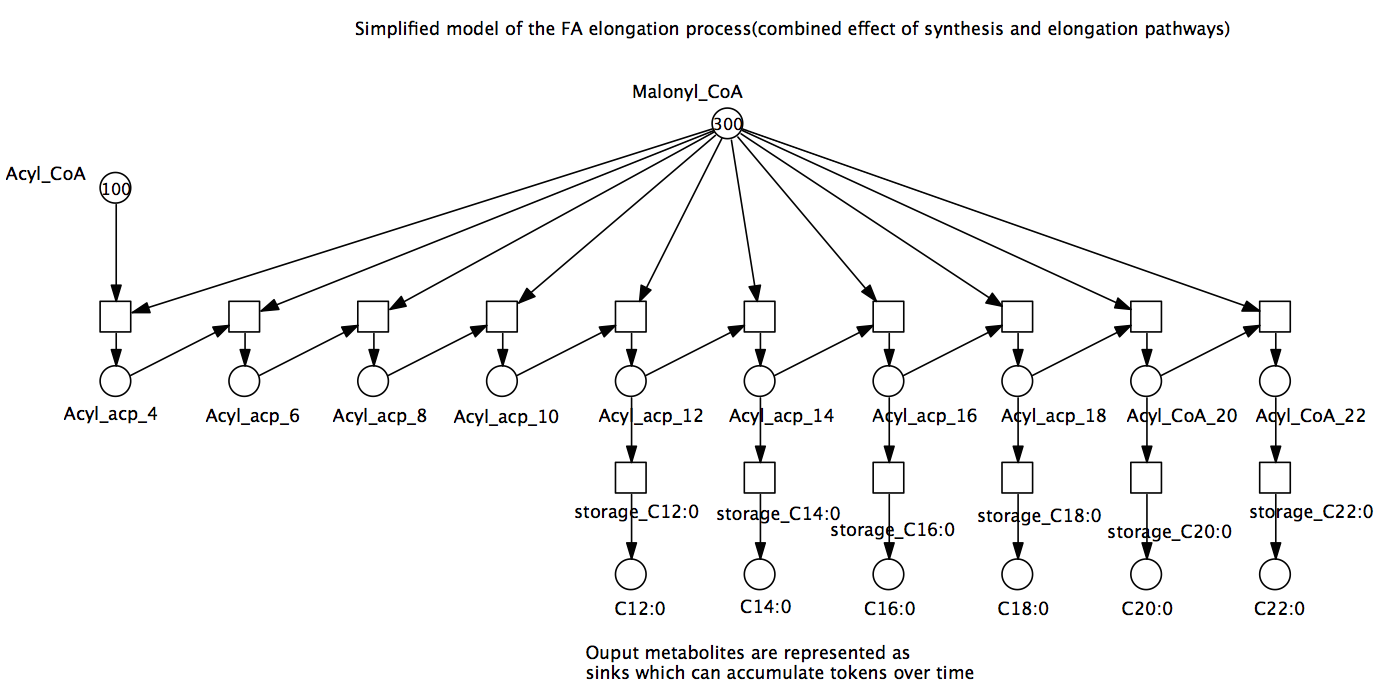
\includegraphics[width=1.0\textwidth]{fa_elongation_full}
\caption[Petri Net implementation(basic model)]{Petri Net
  implementation of the basic model as described in the main text}
\label{fig:fa_elongation_full}
\end{figure}


Observing the execution pattern of the basic net model we notice an
execution pattern which leads to an elegant view of the system as a
series of binary probabilistic decisions or Bernoulli trials. The way
the inputs of the model are set up, at the start of the model
execution only the initial transition producing the first product $C_4$ is
enabled. If we consider that after this transition fires (since its
the only one enabled) it
will only fire again after its initial product has reached a sink then
at each point only one token is travelling through the net. This token
goes through an iteration of binary decisions: stay at current length
\textit{or} continue to form a longer
FA. More formally as the token gets
transformed to an intermediate product there are only two transitions
enabled: the transition taking it to the next longer intermediate and
the transition taking to be stored at its current length(Figure~\ref{fig:binary_decision}). Let these
two transitions be $t_1$ and $t_2$ respectively. According to
the operational semantics of Stochatic Petri Nets(see Methods section)
a wait time is sampled for each of the enabled transitions from a
negative exponential distribution with rate the value of the rate
function of the
transition. In this case the rate function of the two transitions are
constants(see assumptions) $\lambda_{t_1}$ and $\lambda_{t_2}$. Since
we know that one of the reactions will fire we can say that the
firing probabilities of the two transitions or the probabilities of
the token's decisions are:

\begin{align*}
P(staying)& =P(t_1) = \frac{\lambda_{t_1}}{\lambda_{t_1} + \lambda_{t_2}}\\
P(continuing) & = P(t_2) = \frac{\lambda_{t_2}}{\lambda_{t_1} + \lambda_{t_2}} = 1 - P(t_1)\\
\end{align*}


\begin{figure}[htbp!]
\centering
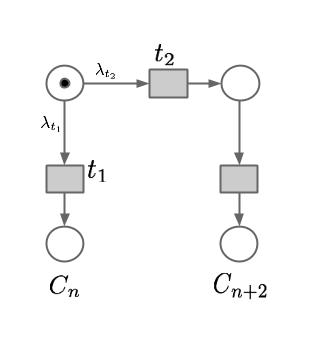
\includegraphics[width=0.5\textwidth]{binary_decision}
\caption[Binary stay-continue decision]{Binary decision at a
  particular point in the execution.}
\label{fig:binary_decision}
\end{figure}

In other words this is a Bernoulli trial with probability of success
$p = P(t_1)$. Since we only care about the outputs at the end of the
execution and not the timeframe of the process from start to finish
then only the ratio of these two successive transitions rates is
important and not their absolute numbers. Then the entire journey of a token through the network
from the initial $C_4$ product until it reaches a sink and gets stored
can be thought of a series of Bernoulli
trials(Figure~\ref{fig:trials}). Then the entire stochastic process
can be thought of a sequence of successive realisations of this series
of trials with tokens travelling through the net one
after the other with each one going through the series of decisions
or Bernoulli trials. The initial assumption that only one token
travels through the net at each time can in fact be dropped since the
output of the net only depends on the ratios of the pair of
transitions representing each binary decision. I just chose to have it
because this leads to the nice picture of the successive realisations
of chains of Bernoulli trials which is intuitive for illustration
purposes.
It is also interesting to note how this binary decision
corresponds to a conflict between two events that share pre-conditions
which create non-determinsim through a race condition between the two
depdendent events. This 'conflict' which represents this decision
process is captured inherently in the structure and semantics of Petri
Nets.

\begin{figure}[htbp!]
\centering
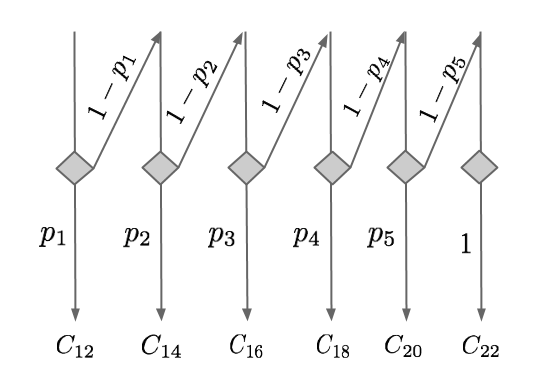
\includegraphics[width=0.55\textwidth]{trials}
\caption[Stochastic proces as a series of Bernoulli trials]{The entire
stochastic process a series of Bernoulli trials.}
\label{fig:trials}
\end{figure}

Each realisation of the stochastic process described by the Petri Net
model which is itself a series of successive realisations of series of
Bernoulli trials will have different outputs. While SNOOPY is a great
tool for the visual side of things, creating the model and animating
them, in order to be able to execute the model many times to get
output profiles we needed a programmatic solution. I wrote code in
Python that can read a model, execute it once or many times, and write
out the results. For the description of the model I used the PySCeS
model description language for biochemical systems which is aimed at
the Python language. The reactions are
defined in the standard chemical notation and since this corresponds
exactly to Petri Net transitions it was easy to load the description
into an appropriate Petri Net representation(Figure~\ref{fig:code}).

\begin{figure}[htbp!]
\centering
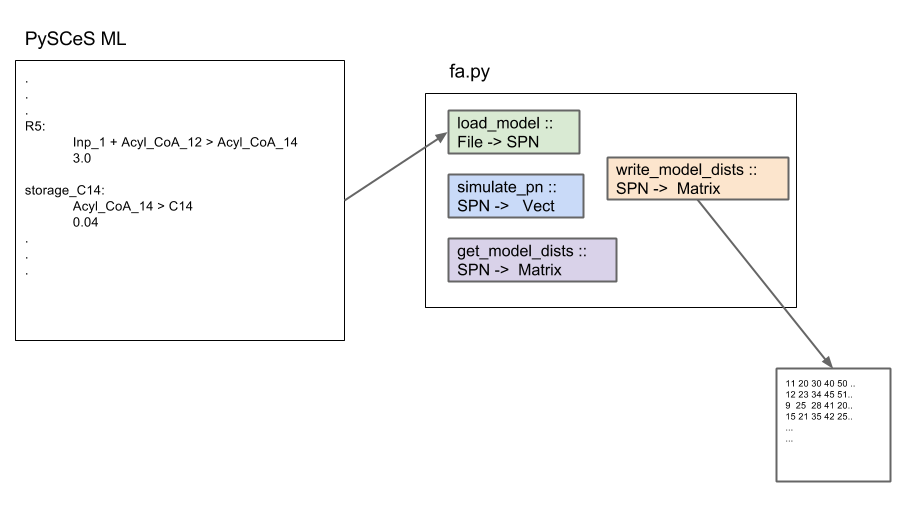
\includegraphics[width=1.0\textwidth]{code}
\caption[Workflow]{Structure of the code and workflow}
\label{fig:code}
\end{figure}


\subsection{Model parameters}
In the previous section I described the building of the basic model
based on the goals and assumptions of the study. The elongation aspect
that we are interested in was reduced down to a sequence of successive
series of Bernoulli trials that determine the length that a FA will
stop its elongation at. The interesting parameters of the model, the
ones that will affect the output, are the success probabilities for
the stay-continue decisions for FA intermediaries with lengths
$[C_{12}, C_{22}]$ since they are ones that have sinks. In this
section two methods for the identification of these parameters for
tuning the model so that its execution is biologically valid are
presented. They both rely on experimental data from an MS study that
contains relative MS spectra intensities for a number of lipid
products extracted from cells. The aim of the study for which the
experiment was conducted was to identify the effect of some treatment
in lipid products so it included 90 samples from control and treatment
(at different levels) individuals. Here we are only interested in creating a null
model so only the 30 samples from the control individuals in the
experiment were retained for
the purposes of parameter tuning.

The outputs of the net model are integer number of tokens accumulated
at each of the sinks or FA of different lengths while the experimental
data are relative intensities which are continuous numbers. In order
to be able to compare the two for the tuning of the parameters the
experimental data were transformed from relative intensities to
relative absolute numbers. The transormation of a sample of relative
intensities $\mathbf{s} = \{s_1, s_2, s_3, s_4, s_5, s_6\}$ became a
transformed sample $\mathbf{ts} = \{ ts_i | ts_i = \lfloor s_i /
min(\mathbf{s}) \rfloor \}$.
 Since we are only interested in the
relative proportions of the outputs going from relative intensities to
relative numbers should not affect the outcome. The data can then be
seen as different realisations of the stochastic process described by
the real model that acts in nature. The attempt is then to tune our
model to be as close to the real model as possible by trying to tune
the proportions of the outputs of our model to match the proportions
of the outputs by the real model represented in the experimental
data. This is  classical Machine Learning formulation of the inverse
problem(Figure~\ref{fig:ml}). In this section I first present a method to get point
estimates and then profiles for the success probabilities parameters of the series of Bernoulli
trials representing the chain of decisions for a token travelling
through the net.

\begin{figure}[htbp!]
\centering
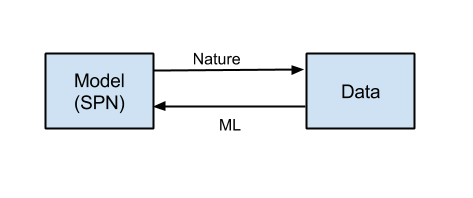
\includegraphics[width=0.5\textwidth]{ml}
\caption[ML inverse problem formulation]{ML inverse problem formulation}
\label{fig:ml}
\end{figure}



\subsubsection{Point estimates}
The data more formally are a matrix $D$ with an element $D_{ik}$ being
the number of tokens accumulated in the $k$-th FA in the $i$-th
sample or realisation of the process. Since we have multiple
realisations of Bernoulli trials the success probabilities can also be
though of as success probabilities in binomial distributions. The
Maximum Likelihood point estimator for binomial success probabilities
is given for the $i$-th decision corresponding to the $i$-th FA,
\begin{equation*}
\hat{p_i} = \frac{k_i}{n_i}
\end{equation*}
, where $k_i$ is the number of successes and $n_i$ is the number of
trials. If we extract information about the number of successes and
number of trials for each binary decision in the process from the data
that are different realisation of the process then we can
straightforwardly compute the success probabilities we are after.

If we a take a specific sample (a row from data matrix $D$) then the
number of successes for an FA are simply just the number of tokens of
that FA in the sample since those are the tokens that when faced with
the decision of whether to get stored as that FA or continue to form
longer FAs they chose the former. Success and failure are arbitrarily
assigned to staying and continuing respectively. The number of trials
is the number of all the tokens that reached that FA intermediary, both
the ones that stayed \textit{and} the ones that continued. Since this
is an iterative process the ones that continued are the number of
tokens that made it to the sinks after the FA(the ones on the right as
we look at the Petri Net model picture,
Figure~\ref{fig:fa_elongation_full}). To illustrate this consider a
sample which could be a row from our data matrix $D$: $\{C_{12}=5,
C_{14}=10, C_{16}=34, C_{18}=23, C_{20}=3, C_{22}=5\}$. The ML
estimator for the $i$-th FA product in that sample will be:
\begin{equation*}
\hat{p_i} = \frac{C_i}{\sum_{n \geq i} C_n}
\end{equation*}
The success probabilities $p_1$ to $p_6$ for the above sample, with $p_1$ corresponding to
the first binary decision and $C_{12}$, $p_s$ to the second decision
and $C_{14}$ and so on, are:
\begin{align*}
\hat{p_1} & = 5/(5+10+34+23+3+5) = 0.0625\\
\hat{p_2} & = 10 / (10+34+23+3+5) = 0.1333\\
\hat{p_3} & = 34 / (34+23+3+5) = 0.523\\
\hat{p_4} & = 23 / (23+3+5) = 0.742\\
\hat{p_5} & = 3 / (3+5) = 0.375\\
\hat{p_6} & = 1
\end{align*}
This is for one sample but since all the samples are from the same
population(controls) we can combine the successes/trials data from all
samples and generalise the ML success probability estimation for the
$i$-th FA products as:
\begin{equation*}
\hat{p_i} = \frac{\sum_k D_{ki}}{\sum_k \sum_{n\geq i} D_{kn}}
\end{equation*}
We assume that the columns of data matrix D are ordered according to
the order of FAs in the system.

The success probabilities ML estimators from the real experimental dataset
can be seen in Table~\ref{tab:param_estimates}.

\begin{table}
\centering
    \begin{tabular}{ccc}
    Parameter & Value \\
    $p_1$ &  0.0003000656 \\
    $p_2$ & 0.0400323889\\
    $p_3$ &  0.8235217126\\
    $p_4$ &  0.9888339514\\
    $p_5$ &  0.778597786 \\
    $p_6$ &  1.0
    \end{tabular}
\caption{Success probabilities}
\label{tab:param_estimates}
\end{table}
Since
we do not care about the timeframe of the process but rather at the
output at the end the relative proportions of the transitions
participating in a binary decision are what is important therefore we
can use the calculated success probabilities as the rates of the
transitions related to the binary decision. So for example since
$\hat{p_3}\approx0.82$ then the rates of the transitions corresponding to the
binary decision for the 3rd FA, $C_{16}$, will be: rate of transition
for $C_{16}$ storage (success) $0.82$ and rate of transition for
$C_{18}$ formation (failure) $0.18$($1-P(success)$).


\subsubsection{Profiles}
In the previous section I derived point estimates for the success
probabilities guiding the binary decisions taking place during the
elongation process. I did that by considering the success
probabilities that maximise the likelihood function $L(D|p_i)$ for
the $i$-th FA and data $D$ being the number of successes and number of
trials. In this section I will present a likelihood function for the
entire process which comes naturally by thinking of the process as
before as a sequence of series of Bernoulli trials. I then use this
likelihood function to get the profiles of the parameters of interest.


The data from one of the samples can be seen as one realisation of the
stochastic process with the numbers of tokens at each FA being the
outputs of the series of Bernoulli trials that make up one realisation
of the entire process. Each series of Bernoulli trials describes the
journey of one token through the net which ends when it finds a
sink. If for example the token ends up at the third sink that means
that the outcome of the series of Bernoulli trials was: fail, fail,
success. Therefore the data consisting of the number of tokens that
ended up at each FA gives us a history of the series of trials that
happened during that realisation of the process. Consider the
following sample $\{C_{12}=5, C_{14}=10, C_{16}=34, C_{18}=23,
C_{20}=3, C_{22}=5\}$ which is one realisation of the process from
the start until reaching a dead-state. The numbers tell us the 'fate'
of each of the tokens that went through the net during that
realisation of the process, 5 tokens made the decision to stay at the
first trial- [success]- , 10 tokens made a decision to continue on the
first decision and then to stay on the second decision- [fail,
sucess]-, 34 tokens continued on the first two decision and stayed on
the third- [fail, fail, success], and so on. We can therefore calculate
the probabilities for each FA product sinks as follows:
\begin{align}
P(C_{12}) &= p_1 \nonumber\\
P(C_{14}) &= (1-p_1)p_2 \nonumber\\
P(C_{16}) &= (1-p_1)(1-p_2)p_3 \nonumber \\
P(C_{18}) &= (1-p_1)(1-p_2)(1-p_3)p_4 \nonumber\\
P(C_{20}) &= (1-p_1)(1-p_2)(1-p_3)(1-p_4)p_5 \nonumber\\
P(C_{22}) &= (1-p_1)(1-p_2)(1-p_3)(1-p_4)(1-p_5)p_6 \nonumber\\
\label{eq:param_cor}
\end{align}
The entire process can then be seen as a multinomial draw with 6
outcomes,  $\{C_{12}, C_{14}, C_{16}, C_{18}, C_{20}, C_{22}\}$, with
their respective probabilities given above and with the number of
trials being the number of tokens that ended up in sinks for that
particular realisation of the process. This gives the likelihood
function of the data given the success probabilities as
probability mass function of the multinomial distribution:
\begin{equation*}
L(D|\mathbf{\theta}) = f(C_{12},\dots, C_{22}; n ; P(C_{12}), \dots,
P(C_{22})\}) =
\end{equation*}

Using the likelihood function for the entire process we can find the
posterior of the initial success probabilities $p_1$ to $p_6$,
\begin{equation*}
P(\{p_i\} | D) \sim L(D | \{p_i\}) P(\{p_i\})
\end{equation*}
where the data $D$ is simply the outputs of one realisation of the
process or the counts at each sink and $P(\{p_i\})$ are the priors of
the parameters. If we assume uniformative priors the above parameter
posterior simply becomes: $P(\{p_i\} | D) \sim L(D | \{p_i\})$. Since
the parameters are not exactly the parameters of the multinomial but
they are only related through Equations~\ref{eq:param_cor} an analytic
solutions is not very attractive but since it is still a small problem
we can resort to a simple simulation scheme to sample from the required
posterior. I used the standard Metropolis-Hastings MCMC method to
sample from the posterior as given above starting from a random point
in parameter space and a symmetric normal proposal distribution with
mean the previous accepted guess and an arbitrary chosen variance. The
MCMC traces and the histograms of the samples obtained from the
posteriors can be seen in Figure.


\subsection{A stochastic $\pi$-calculus implementation}
In this section I present a stochastic pi-calculus version of the
model which is specifically written in its SPiM variant which extends
the traditional pi-calculus first by introducing explicitly time which
is needed for quantitive analysis of biochemical networks and also by
adding operational semantics in terms of an Abstract Machine and a
graphical representation language. The SPiM code is given for the
processes making up the system to introduce further some of the
concepts of the SPiM language. For more information about the SPiM
language.

The SPiM graphcal representation of the model can be seen in
Figure~\ref{fig:spim_graph}. Each component of that graph is a
stochastic pi-calculus process and edges between them indicate that
one one of them can evolve into the other. The nature of the model is
different from the equivalent model given in the previous section. The
evolution of every species represented by a stochastic pi-calculus
process which is defined independently. We start the computation by running 100
\texttt{Acyl\_CoA} processes and 30 \texttt{Malonyl\_CoA} processes:

\begin{verbatim}
run(100 of Malonyl_CoA() | 30 of Acyl_CoA())
\end{verbatim}

The initial reaction of the system creating the $C_4$ product is represented as
communication by channell \texttt{form6} between \texttt{Acyl\_CoA} and
\texttt{Malonyl\_CoA} processes. Once the communication happens the
\texttt{Acyl\_CoA} process evolves into the  \texttt{Acyl\_CoA\_4}
process while \texttt{Malonyl\_CoA} process goes to the empty
process(gets consumed). After that all the processes corresponding
FAs between $C_6$ and $C_{10}$ only have one communication option,
communicate via the appropriate channell with a \texttt{Malonyl\_CoA}
process and then evolve into a process corresponding to a longer
FA. For example process \texttt{Acyl\_CoA\_8}:

\begin{verbatim}
and Acyl_CoA_8() = ?form10; Acyl_CoA_10()
\end{verbatim}

After that all the processes corresponding to intermediaries for longer
than $C_{10}$ FAs have two communication options corresponding to the familiar
stay-continue stochastic decision that we have seen in the previous section, they
can either communicate with a \texttt{Malonyl\_CoA} process and evolve
into a process corresponding to a longer FA while the
\texttt{Malonyl\_CoA} process terminates or do a delay and evolve into
their corresponding FA product. The FA products which are modelled as
empty processes could have been ignored since they do not interact
further with any other processes but they were kept there
intentionally to keep track of their numbers.

\begin{figure}[htbp!]
\centering
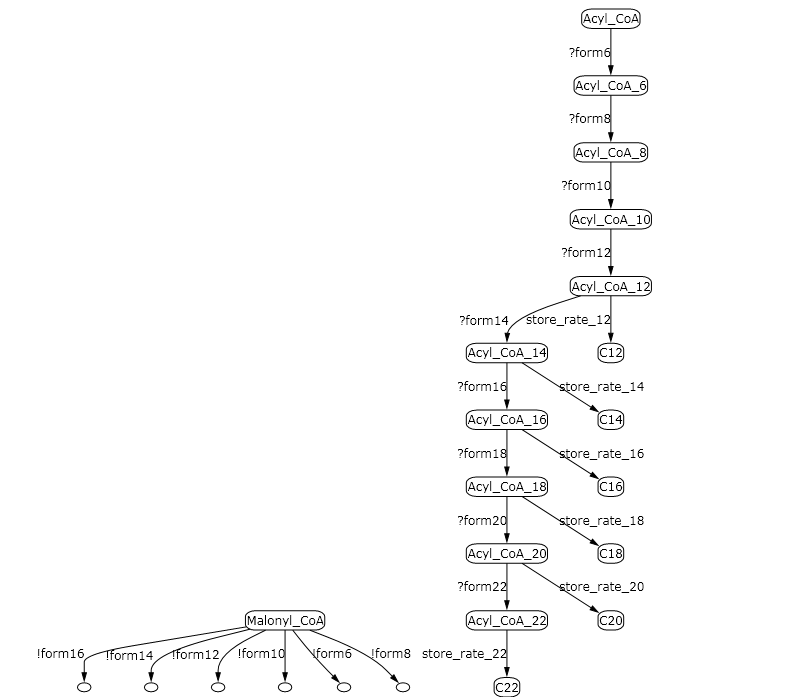
\includegraphics[width=1.0\textwidth]{spim_graph}
\caption[SPiM graph]{SPiM graph}
\label{fig:spim_graph}
\end{figure}

\begin{verbatim}
let Malonyl_CoA() =
(
	do !form6; ()
	or !form8; ()
	or !form10; ()
	or !form12; ()
	or !form14; ()
	or !form16; ()
)
and Acyl_CoA() = ?form6; Acyl_CoA_6()
and Acyl_CoA_6() = ?form8; Acyl_CoA_8()
and Acyl_CoA_8() = ?form10; Acyl_CoA_10()
and Acyl_CoA_10() = ?form12; Acyl_CoA_12()
and Acyl_CoA_12() =
(
	do ?form14; Acyl_CoA_14()
	or delay@store_rate_12; C12()
)
and Acyl_CoA_14() =
(
	do ?form16; Acyl_CoA_16()
	or delay@store_rate_14; C14()
)
and Acyl_CoA_16() =
(
	do ?form18; Acyl_CoA_18()
	or delay@store_rate_16; C16()
)
and Acyl_CoA_18() =
(
	do ?form20; Acyl_CoA_20()
	or delay@store_rate_18; C18()
)
and Acyl_CoA_20() =
(
	do ?form22; Acyl_CoA_22()
	or delay@store_rate_20; C20()
)
and Acyl_CoA_22() = delay@store_rate_22; C22()
and C12() = ()
and C14() = ()
and C16() = ()
and C18() = ()
and C20() = ()
and C22() = ()

run(100 of Malonyl_CoA() | 30 of Acyl_CoA())
\end{verbatim}


\section{Extended model of FA synthesis}
In the previous section I presented a Petri Net and stochastic
pi-calculus implementations of a
simplified view of FA elongation/synthesis. In this section I
will present a Petri net implementation of an extended model which
captures one of the main control regulatory mechanisms between FA
biosynthesis and other general metabolic
machinery of the cell. The first and commited step in the FA
biosynthesis pathway is the conversion of acetyl-CoA to Malonyl-CoA
through the action of acetyl-CoA carboxylase. Acetyl-CoA carboxylase
is inactivated by AMPK protein kinase in mammals. In the well-fed
state AMPK is itself inactivated which leads to an increase in the
flow of Acetyl-CoA to Malonyl-CoA and since this is an irreversible
reaction to the FA biosynthesis pathway. 
Also in conditions of high glucose
concentration isocitrate dehydrogenase is inhibited so Acetyl-CoA only
does the first step of the Krebs cycle when Citrate is produced. Since
Citrate cannot go any further in the cycle it starts to accumulate
until it starts to diffuse from the mitochondrion into the cytosol
where it becames Acetyl-CoA again and acts as precursor for FA
biosynthesis. The net effect of this two is that more Acetyl-CoA will
flow towards the FA biosynthesis than go towards the
Kreb cycle and the Respiratory chain to produce energy because the
immediate energy requirements are low(high ATP).

\citet{nielsen2009systems} experimentally confirmed that
this regulatory mechanism is conserved in yeast through the action of
Snf1 which the yeast analog of the mammalian AMPK and they also
produced Flux Balance Analysis systems biology models to capture the
change in flows in the system throught the action of protein kinase
Snf1. Here we provide a Petri Net implementation of the above
regulatory scheme as an extension to the basic model we presented
in the previous section.

\subsection{Petri Net implementation}
The Petri Net implementation of the above mentioned regulatory
mechanism as an extension to the basic model presented before can be
seen in Figure~\ref{fig:pn_ext}. The net starts with an empty
transition feeding into glucose which can be thought of as an
interface to the environment. That could for example be used to model
glucose intake from the diet. Then after that the action of every pathway
is condensed into a single transition except FA
biosynthesis/elongation for which we use the basic model developed
previously. After the initial glucose intake transition, glucolysis is
represented by a transition from Glucose to Pyruvate and then
Acetyl-CoA which plays the central role in this regulatory
mechanism. Acetyl-CoA has a decision of whether to flow towards FA
biosynthesis represented by transitions to place \texttt{FAsyn}
or flow towards the TCA cycle and further energy production which is
represented by a transition to the \texttt{TCA}
place. The \texttt{TCA}  place represents the combined
effect of the TCA cycle and the respiratory chain which has as an
ouput 30 molecules of ATP. ATP can then be consumed by taking part in
a transition without any post-places. ATP consumption could for
example be used to model various energy requirements. The FA biosynthesis/elongation
process is represented as before with the only difference
being that it now only has a single input which then leads to the two
inputs used in the basic version of the model. 
The main regulatory mechanism comes by making ATP a pre-place for the
Acetyl-CoA transition to \texttt{FAsyn} so that ATP levels can
influence the rate of that transition and hence the flow towards FA
biosynthesis. 

\begin{figure}[htbp!]
\centering
\includegraphics[width=1.0\textwidth]{pn_ext}
\caption[Extended Petri Net model]{An extended version of the model}
\label{fig:pn_ext}
\end{figure}


\subsection{Model Parameters}
In this section I present a way to contstruct the
rate functions for the transitions out of Acetyl-CoA in order to get
the required regulatory behaviour based on ATP levels and a way to
find the rate parameters for the transitions from the \texttt{FAsyn} place
to the two main input points for the FA synthesis/elongation process.

Since we have not modelled enzymatic
activity explicitly but only through the transition rates, the effect that ATP has on the enzyme responsible
for the flow of Acetyl-CoA to FA synthesis will have to become an effect
on the rate of the corresponding transition. In order to introduce
that effect the rate function for the transition taking Acetyl-CoA to FA biosynthesis
becomes an increasing function of ATP. That by itself
is not enough though since at high ATP levels the reaction rate not only
needs to be high but crucially higher than the TCA transition rate in order to
make the flow towards FA biosynthesis more favorable when Acetyl-CoA
is faced with the TCA/FA biosynthsesis decision. So again the
important thing here, since we do not care about the timeframe of the
process, is the ratio between these parameters. In order to achieve
that we can set up a basal rate for the two alternatives for a
base level of ATP for which they are both equally likely to
happen. Any deviations from that balanced level and the flow towards
FA biosynthesis becomes more or less likely. Let us consider a
constant base level of $ATPb$ ATP molecules and a variable $ATP$ for the number
of ATP molecules at any given time during the execution of the
model. An example of rate functions that meet our requirements are:
$\lambda_{TCA} = ATPb^{k}$ and $\lambda_{FAsyn} =
ATP^{k}$. When $ATP=ATPb$ the transition rates are equal so the
Acetyl-CoA flows with equal likelihood to TCA and FA
biosynthesis. The strength of the response to deviations is then:
\begin{equation*}
\left ( \frac{ATP}{ATPb}\right)^{k}
\end{equation*}
We can control the strength of the response by tuning the $k$
parameter. For linear responses for example we can set $k=1$ which
will mean that a 2-fold increase in the ATP level from its base rate
results in a doubling of the 
rate of the transition towards FA biosynthesis while the rate towards
TCA remains constant.

For the transition rates from \texttt{FAsyn} we can make a simple
stoichiometric argument to find the correct ratio between them that
will guide the flow towards those two input points of the FA
synthesis/elongation process. For every $C_2$ concatenation step we
need one Malonyl-CoA so for example if the process does 7 steps to
reach the $C_{16}$ then we would need 7 Malonyl-CoAs and 1
Acetyl-CoA. Since it is a stochastic process however we do not know in
advance how many steps each token will take through the net. We can
however find the expectation of the number of steps:
\begin{equation*}
E(steps)=\sum_{4 \leq i \leq 9} i \times P(i)
\end{equation*}
So on average we need $E(steps)$ Malonyl-CoAs for every one
Acetyl-ACP. We can set the transition rates towards these two starting
points to reflect that:
\begin{align*}
\frac{\lambda_{Malonyl\_CoA}}{\lambda_{Acetyl\_CoA}} = E(steps)
\end{align*}

\subsection{Model Execution and discussion}


\chapter{Discussion}

% **************************** Define Graphics Path **************************
\ifpdf
    \graphicspath{{Discussion/Figs/Raster/}{Discussion/Figs/PDF/}{Discussion/Figs/}}
\else
    \graphicspath{{Discussion/Figs/Vector/}{Discussion/Figs/}}
\fi

This section is divided into two logical parts. The first two
sections are commentary and critique on firstly the created model and
secondly the languages we used to capture the model. The last section
takes the form of perspectives and future directions of both the
language methodology and our developed model.

\section{Simplified model and accuracy of description}
In this work we created an abstract simplified reaction-centric model
of the biosynthesis and elongation
process that takes place in the cytosol and ER. The model developed captures the defining high-level
characteristics of this process accurately. The developed model allows
us to observe the series of elongation steps and get distributions of
outputs of FA products that can be compared with real experimental
datasets as we have done in section Results. We have also shown how
we can tune the parameters of the model in the presence of such datasets. The assumptions we made however
for the construction of the model make it biochemically
inaccurate. So while it might provide a high level view of the model
in a conceptually clear way it does not reflect the
actual biochemical process that takes place inside the cell. All the
reaction rate functions were assumed to be constant and treated as
probabilities without regarding enzymatic activity and numbers of
molecules of the
reactants. In fact all the concatenation steps of the process involve
the activity of the same enzymes so the basal reaction rates
(probability of reaction between two reactant molecules) should be the same for
all elongation steps with maybe some slight differences due to the different interaction between the enzymes and FA with different lengths. There must be then some other underlying
biochemical mechanism that
gives rise to the probabilistic interpretation we provided through our
model. Each concatenation step was also considered as a single
reaction instead of the four that it actually takes. This assumption does not pose a big problem for the
biochemical validity of the model if the stoichiometries and enzyme
activities participating in the reactions are considered
carefully. The other big simplification was the combination of the two
pathways acting together for the elongation of FAs, FA biosynthesis in
the cytosol
for FA lengths up to 16 and FA elongation in ER for longer FAs. The
transportation between the cytosol was not considered. Transportation
could be added with the current methods on an ad-hoc basis by
considering for example a delayed transition between $C_{16}$ and
$C_{18}$ (transportation delay) or having two $C_{16}$ places, one
cytosolic and one in ER, and a transition between them encoding the
transportation event.

In the extended model we considered the relation between different
pathways in the metabolic machinery of the cell. We only wanted to
investigate the communication between the interfaces of the different
pathways so we represented pathways by one transition and explicitly
only the metabolites that provide the communication interface between FA biosynthesis/elongation process and
other pathways. So for example the entire TCA cycle and respiratory chain
responsible for the production of energy was represented as one transition with
only ATP as output as that is the point of
communication with the FA biosynthesis process. ATP is required in the
conversion of Acetyl-CoA to Malonyl-CoA for the first committed step
towards FA biosynthesis and also acts as a regulation metabolite of
the AMPK protein kinase that inhibits this step. Also this interaction
was represented as a single step while in reality it goes through the
AMPK protein kinase. Again transportation between the compartments
that in this case also include the mitochondrion is not included and
Acetyl-CoA is represented by a single place. An interesting aspect of
our model is that we can also capture the communication between the
pathways and the environment for example by setting the rate for
glucose intake or the rate of ATP consumption.

In a way our models do not completely fall into the bottom-up or
top-down approaches to model construction. We started from some
knowledge of the system to construct the model in the first place
(top-down) but then experimental data guided some of the decisions in
the model simplification. In the end the FA biosynthesis/elongation
simplified model can provide accurate description and a mechanistic model for the reproduction of
measurable quantities but not a mechanistic model for the underlying
biochemical process. We still consider this a reaction-centric model
though despite the fact that the Petri Net transitions do not exactly
correspond to accurate biochemical reactions because the main events of the model are the
transformations of species from one form to the other.

\section{Description languages}
One of the project goals was also to investigate modelling methods
for a suitable language to describe the reaction-centric view of lipid
metabolism. We particularly focused on Petri Nets that were the main
language used but we also provided an alternative stochastic
pi-calculus (SPiM) implementation of the basic model.

Petri Nets have an attractive graphical notation language that
captures the main
characteristics we identified in lipid metabolism that served as
motivation for this reaction-centric view: iterative conversion
processes and probabilistic decisions. There is also a very natural
correspondence between Petri Net transitions and reactions. The
behaviour of the net is described with formal operational semantics
that captures this reaction-centric view since the transition is the
main component in the evolution of the computation. Because of the
similarity with the traditional biochemical view of the system and the
static diagrams used to described it we can think of Petri Nets as a
dynamic executable version of the KEGG diagrams. Petri Nets are also
expressive enough to allow us to move up or down the abstraction
scale. For example in the extended net model we had places
corresponding to entire pathways or places that were placeholders for
the flow towards a specific pathway (\texttt{FAsyn} place in
Figure~\ref{fig:pn_ext}). The formal operational semantics have a
graphical equivalent in the form of the token game that can provide
intuition in the workings of a pathway or network. There is a long
tradition of using Petri Nets so there exist many tools to 'draw' nets
and play the token game. In this work we mainly focused on
quantitative analysis of stochastic Petri Nets but the dynamic picture
is only part of the strength of Petri Nets. Their formal specification
allows for qualitative static topological analyses that yield the
same insides as standard techniques in the field like Elementary Modes
analysis. Another topic that we do not address here but it is of
particular interest especially as the models grow in size is the model
checking ability we have with the use of Petri Nets. We can use model
checking techniques for example to explore qualitative and quantitative
static and dynamic properties of systems. \citet{gilbert2007unifying}
go as far as to provide a unifying framework for both qualitative and
quantitative analysis of biochemical networks captured with the Petri
Net language. It is interesting that we can use the same language to
analyse and describe features of systems that are usually captured
with different approaches. One major drawback of Petri Nets is that they
are monolithic. Models cannot be decomposed to smaller parts in order
for example to abstract away non-important details of parts of the
process that are not of immediate interest. We did this informally in
the extended version of the model by defining entire pathways as
transitions and by including only the metabolites that provided the link
to other pathways. This is not captured formally though in the
language. The inherent coupling with the chemical reaction view makes
the constructed models grow linearly with the number of
reactions. This is not a major problem for metabolic pathways because of
the iterative chain of conversion that usually takes place. For
larger systems however with combinatorial interactions between species
there are scaling issues (See Future perspectives for some thoughts on
decomposability and scalability).

Stochastic pi-calculus and specifically SPiM are more detached from
the standard biochemical graphical notation. Each component of the
system is defined independently in contrast to the Petri Nets where the
main unit of definition are the transitions corresponding to the
reactions. Their operational reduction semantics are however defined in terms
of communication between the components that correspond to the
reactions. It is particularly suited to metabolism because metabolic
pathways usually involve linear series of conversions. These linear
series of conversion can be encoded with the sequential operator of
the calculus that defines state changes of a component after
communication actions (reactions). The other characteristic we are
interested in, decisions, is also captured nicely with the choice
operator of the calculus that provides non-determinism. Another
advantage of stochastic pi-calculus over Petri Nets is the
decomposition that is inherent in the syntax/semantics. This coupled
with the fact that the model size grows linearly with the number of
species (instead of reactions) could make them more attractive for
larger networks.



\section{Future perspectives}

\subsection{Modelling and experimental validation}
In this section we present some possible future directions for our
constructed models and experimental validation.

Using the already constructed models as a scaffold we can expand
them to include interactions with other pathways. In this work we
concentrated on even-chain saturated FAs but these are not the only FA
products. FAs can get modified after creation not only but the
elongation pathway we considered but by adding double bonds at one
(monounsaturated) or many (polyunsaturated) places in their CH
tails. Then these FA products of different lengths and numbers of
double bond combine as building blocks to form more complex lipid
products like triacylglycerols (TAGs) and diacylglycerols (DAGs). DAGs
and TAGs contain a headgroup and two or three FAs
respectively. Following from our high level view of FA
biosynthesis/elongation we can derive probability equations for these further
modifications and complex formations. Our current
modelling methods are suited to this kind of system. For example
if we also had some experimental data about the frequencies of the
triplets or pairs of FAs found in TAGs and DAGs respectively we could
extend the model by making the current sinks of the system feed into
transitions for complex formation using the frequencies to infer the
probabilities. Perhaps we could start from yeast that only has
mono-unsaturated FAs to limit the combinatorial space in complex
formation \cite [] {nielsen2009systems}. Yeast is a good choice for a
model organism as it produces complex lipids like other animals but
without taking Polyunsaturated FAs from the diet.
Production and modelling the net forward direction is only part of
the story however and the corresponding catabolic processes are
equally important and the balance between them one of the major goals
of the interplay and control between different parts of the metabolic
machinery. For example we can add degradation of
FAs. Finally as an extension to our model with control we could add
other control mechanisms. The control of Acetyl-CoA flow to FA
biosynthesis through ATP and AMPK is only one point of control. The
production of $C_{16}$ molecules also inhibits the flow to prevent the
accumulation of FAs for example.


In order to validate our modelling strategy we need to compare its execution to real data. We have done
that for our basic model for which we have output real output. It would be interesting to gather experimental data to confirm the
control mechanism between ATP and Acetyl-CoA flow to FA formation. For
example we could use $^{13}C$ metabolite labelling to get time-series
data of the flows. This would allow us to calculate the strength of
the response to ATP change (through TCA activity) in Acetyl-CoA flow towards FA biosynthesis
and would allow us to tune the $k$ parameter we used in our extended
model for the transition from Acetyl-CoA to the \texttt{FAsyn}
place. Having experimental data across different conditions, like we
had for example for our basic model, could provide another useful
dimension to our models. In the Results section we calculated the
model parameters for different clusters of lipid product patterns among the FA distribution under healthy and pathological conditions. By
observing changes in the parameters across conditions we could
pinpoint areas or structures that show behavioural changes in the model. This could lead
to mechanistic understanding of changes that lead to different
conditions and disorders. This would be far more attractive with the
time-series data and the control mechanisms that appear to be the
reasons behind several metabolic disorders. Controlling the diet over
a number of individuals is very hard and dynamic analysis is currently
inaccessible for animals so we could again start with yeast as a
model organism for time-series measurements of metabolites and
flows. Even with our high level
models we could for example calculate the strength response parameter
$k$ across conditions.


\subsection{Language methods}
As we have mentioned in previous sections Petri Nets may not be suited
to larger systems. Even for smaller system they lack the
expressiveness to capture different parts of models at different
levels of abstraction. \citet{DBLP:journals/corr/abs-1304-3121} propose Petri Nets with
Boundaries that can decompose Petri Nets and compositional operators
to define the interconnections between different parts. This approach
has a graphical notation where each part is enclosed in box
representing its boundaries. Each part is itself a Petri Net
consisting of an internal structure of places and transitions as we
have seen before. Every box has output ports that connect it to the
outside world. These ports can be connected with places inside the box
via normal transitions (Figure~\ref{fig:pnb}). The main operator of the algebra is the
synchronisation between these parts for communication. The researchers
have also provided a nice programming language borrowing elements from
functional programming to use along with the
algebra for Petri Nets with boundaries that we believe it is important
in order for these formalisms to be adopted by practitioners. Now this
approach is quite attractive because it allows us to decompose the net
models in an intuitive way and then communication between the
components through the synchronisation operator. In a way it borrows
some of the advantages of process-algebra models while keeping the
vivid graphical notation of Petri Nets. For our purposes of biological
modelling that would mean the different interacting parts could
different pathways or different compartments. If for example we are
only interested in one pathway we could define that part in detail
while define only the interfaces interacting with the outside world
for other pathways. This is what we have done informally in our
extended model but this approach makes it formal. This approach
however has as its main motivation behind the decomposition the
minimisation of state-space for model checking. It will need some
further work for it to be executable and useful for biological
modelling. We are only presenting it here because we believe it is a step
in the right direction.

\begin{figure}[htbp!]
\centering
\includegraphics[width=1.0\textwidth]{pnb}
\caption[Petri Nets with boundaries]{Petri Nets with boundaries. On
  the left two composing parts of the net. Each has its own internal
  net structure and transitions. Some of the places can communicate
  via transitions with the outports of that part(squares at the edge
  of the box). Communication between the two parts happens through
  synchronisation of the outports of the two(picture on the right).}
\label{fig:pnb}
\end{figure}

This is part of a more general attempt to capture hierarchy in
these minimalistic languages for distributed computing. In Petri Nets
with boundaries we can talk at two levels, the local level of the
transitions and state changes inside a box and then the communication
through synchronisation between boxes. Another attempt that falls in
the same category is bigraphs that also has a graphical notation and
the ability to nest structures \cite []
{jensen2004bigraphs}. \citet{degasperi2013process} proposed a process
algebra with hooks that attempts to provide modelling capabilities for
multi-level biological systems and communication operators between the
levels. In our opinion these are steps in the right direction because we
are interested in qualities of biological systems that naturally fall
on different levels. For example in metabolism we might want to talk
about the cross-talk between pathways or communication between cells. We should be able to express these higher level
qualities in terms of the lower level qualities. The language we use
could have primitives to talk about the lowest level, for example
binding between chemical species, and then the language would be
expressive enough to let the modeller/programmer build its own
language that is suited to the problem on top of those primitives.
That way we could
possible have multi-level stratified design of biological systems similar
to computer programs organisation and abstraction \cite [] {abelson1987lisp}.


\include{Conclusions/conclusions}




% ********************************** Back Matter *******************************
% Backmatter should be commented out, if you are using appendices after References
%\backmatter

% ********************************** Bibliography ******************************
\begin{spacing}{0.9}

% To use the conventional natbib style referencing
% Bibliography style previews: http://nodonn.tipido.net/bibstyle.php
% Reference styles: http://sites.stat.psu.edu/~surajit/present/bib.htm

\bibliographystyle{apalike}
%\bibliographystyle{plainnat} % use this to have URLs listed in References
\cleardoublepage
\bibliography{References/references} % Path to your References.bib file


% If you would like to use BibLaTeX for your references, pass `custombib' as
% an option in the document class. The location of 'reference.bib' should be
% specified in the preamble.tex file in the custombib section.
% Comment out the lines related to natbib above and uncomment the following line.

% \printbibliography[heading=bibintoc, title={References}]


\end{spacing}

% ********************************** Appendices ********************************

\begin{appendices} % Using appendices environment for more functunality


\end{appendices}

% *************************************** Index ********************************
\printthesisindex % If index is present

\end{document}
